\documentclass[11pt, a4paper]{article}

% --- 1. Basic Packages ---
\usepackage[utf8]{inputenc}
\usepackage[english]{babel}
\usepackage[T1]{fontenc}
\usepackage{geometry}
\geometry{a4paper, left=25mm, right=25mm, top=30mm, bottom=30mm}
\usepackage{xcolor}
\usepackage{amssymb}
\usepackage[most]{tcolorbox}
\usepackage{float}
\usepackage{rotating}
\usepackage{adjustbox}
\usepackage{makecell}
\usepackage{multirow}
\usepackage{graphicx}
\usepackage{tabularx}
\usepackage{capt-of}
\usepackage{xltabular}
\usepackage{booktabs}
\usepackage{enumitem}
\usepackage{setspace}
\usepackage[none]{hyphenat}
\usepackage[hypertexnames=false]{hyperref}
\usepackage{bookmark}
\usepackage[acronym]{glossaries}
\usepackage{fancyhdr}
\usepackage{chngcntr}

% --- 2. Font setup ---
\usepackage[default,defaultsans,scale=0.95]{opensans}
\newcommand{\sffont}{\sffamily\fontseries{b}\selectfont}

% --- 3. Color and style definitions ---
\definecolor{appleText}{HTML}{1D1D1F}
\setstretch{1.45}
\setlength{\parskip}{0.8em}
\setlength{\parindent}{0pt}
\setlength{\emergencystretch}{2em}
\hyphenpenalty=10000
\exhyphenpenalty=10000
\doublehyphendemerits=100000
\finalhyphendemerits=100000
\setcounter{tocdepth}{2}
\counterwithin{figure}{section}

\newcommand{\symname}[1]{{\sffont #1}}
\newcommand{\symdesc}[1]{#1}

\makeglossaries
\setacronymstyle{long-short}
\newacronym{om}{O\&M}{operations and maintenance}
\newacronym{ess}{ESS}{energy storage system}
\newacronym{ac}{AC}{alternating current}
\newacronym{dc}{DC}{direct current}
\newacronym{pcs}{PCS}{power conversion system}
\newacronym{hmi}{HMI}{human-machine interface}
\newacronym{ups}{UPS}{uninterruptible power supply}
\newacronym{can}{CAN}{controller area network}
\newacronym{spd}{SPD}{surge protective device}
\newacronym{bmu}{BMU}{battery management unit}
\newacronym{pack}{PACK}{battery pack}
\newacronym{bms}{BMS}{battery management system}

\hypersetup{
    colorlinks=true,
    linkcolor=appleText,
    urlcolor=appleText,
    citecolor=appleText,
    linktoc=all,
    pdftitle={eBlock 418 Series Operations and Maintenance Manual},
    pdfauthor={Xi'an Singularity Energy Co., Ltd.}
}

\usepackage{titlesec}
\titleformat{\section}{\Large\sffont\color{appleText}}{\thesection.}{0.5em}{}
\titleformat{\subsection}{\large\sffont\color{appleText}}{\thesubsection}{0.5em}{}

\setlength{\headheight}{11mm}
\setlength{\headsep}{7mm}
\pagestyle{fancy}
\fancyhf{}
\fancyhead[R]{\raisebox{1mm}{
\includegraphics[height=8mm]{logo.png}}}
\fancyfoot[C]{\thepage}
\renewcommand{\headrulewidth}{0pt}
\renewcommand{\footrulewidth}{0pt}

\fancypagestyle{plain}{
    \fancyhf{}
    \fancyhead[R]{\raisebox{1mm}{
\includegraphics[height=8mm]{logo.png}}}
    \fancyfoot[C]{\thepage}
    \renewcommand{\headrulewidth}{0pt}
    \renewcommand{\footrulewidth}{0pt}
}

\begin{document}
\color{appleText}

% ==========================================
% Title Page
% ==========================================
\begin{titlepage}
    \thispagestyle{empty}
    \noindent\makebox[\textwidth][r]{\raisebox{18mm}[0pt][0pt]{
\includegraphics[height=8mm]{logo.png}}}
    \centering
    \vspace*{1.0cm}
    {\Huge\sffont eBlock 418 Series}\\[0.5cm]
    {\Huge\sffont Operations and Maintenance Manual}\\[2cm]

    % Use existing cover image in current directory
    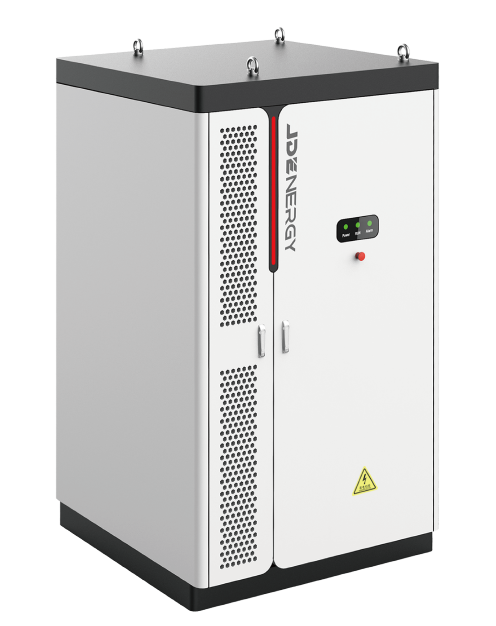
\includegraphics[width=10cm]{e-Block-418-Photo.png} \\[1.2cm]

    \vspace{1.0cm}
    {\large\sffont Xi'an Singularity Energy Co., Ltd.}\\[0.5cm]
    {\color{gray} Version: V1.0 \quad | \quad Date: \today}
\end{titlepage}

% ==========================================
% Table of Contents
% ==========================================
\newpage
\pagenumbering{roman}
\tableofcontents
\clearpage
\printglossary[type=\acronymtype,title=Acronyms]
\newpage
\pagenumbering{arabic}

% ==========================================
% Chapter 1: About This Manual
% ==========================================
\section{About This Manual}
\subsection{Explanation of Symbols}
To ensure the safety of \gls{om} personnel and proper equipment operation, please familiarize yourself with the following symbols:

\vspace{1em}
{\renewcommand\tabularxcolumn[1]{m{#1}}
\begin{tabularx}{\textwidth}{>{\centering\arraybackslash}m{0.16\textwidth} >{\raggedright\arraybackslash}m{0.18\textwidth} >{\raggedright\arraybackslash}X}
\toprule
\textbf{Symbol} & \textbf{Name} & \textbf{Meaning for O\&M Safety} \\
\midrule

\includegraphics[height=3.2em]{warning.png} & \symname{Operation Warning} & \symdesc{Indicates content that, if not properly handled or avoided, may pose a danger to user safety or cause serious damage to the equipment.} \\
\addlinespace

\includegraphics[height=3.2em]{attention.png} & \symname{Attention} & \symdesc{Indicates content that, if not properly handled or avoided, may lead to equipment damage, performance degradation, or other unpredictable results.} \\
\addlinespace

\includegraphics[height=3.2em]{electric.png} & \symname{Electric} & \symdesc{Identifies parts with a risk of electric shock. These areas are hazardous to user safety; \textbf{Do NOT touch} at will.} \\
\addlinespace

\includegraphics[height=3.2em]{temp.png} & \symname{High Temp} & \symdesc{Identifies parts with high-temperature risks that may pose a danger to user safety; \textbf{Do NOT touch} at will.} \\
\addlinespace

\includegraphics[height=3.2em]{ground.png} & \symname{Grounding} & \symdesc{Indicates the connection position for the protective earth (PE) wire to ensure the enclosure is reliably grounded.} \\
\addlinespace

\includegraphics[height=6.2em]{cap_discharge.png} & \symname{Discharge} & \symdesc{High voltage exists when the eBlock is powered on. All operations must be performed by trained professional electrical technicians. To prevent electric shock, touching any live parts is strictly prohibited within \textbf{30 minutes} after disconnecting all power sources to allow for capacitor discharge.} \\
\addlinespace

\includegraphics[height=2.2em]{serial_no.png} & \symname{Serial Number} & \symdesc{Unique identifier for the device.} \\
\bottomrule
\end{tabularx}
}
\vspace{1em}

\subsection{Scope of Application}
This manual is applicable to the routine O\&M of \textbf{eBlock-418 series}. 

It is intended for professional personnel with electrical expertise and experience in power distribution. 

The content of this manual will be continuously updated. There may be slight discrepancies with the actual product; please refer to the physical product and obtain the latest version of the manual through sales channels.

\subsection{Introduction to Energy Storage System}
The electrochemical \gls{ess} consists of the \textbf{Intelligent Energy Block (eBlock)}, the \textbf{Intelligent Energy Link (eLink)}, monitoring platforms, transformers, the utility grid, and associated auxiliary equipment.

\begin{figure}[htbp]
    \centering
    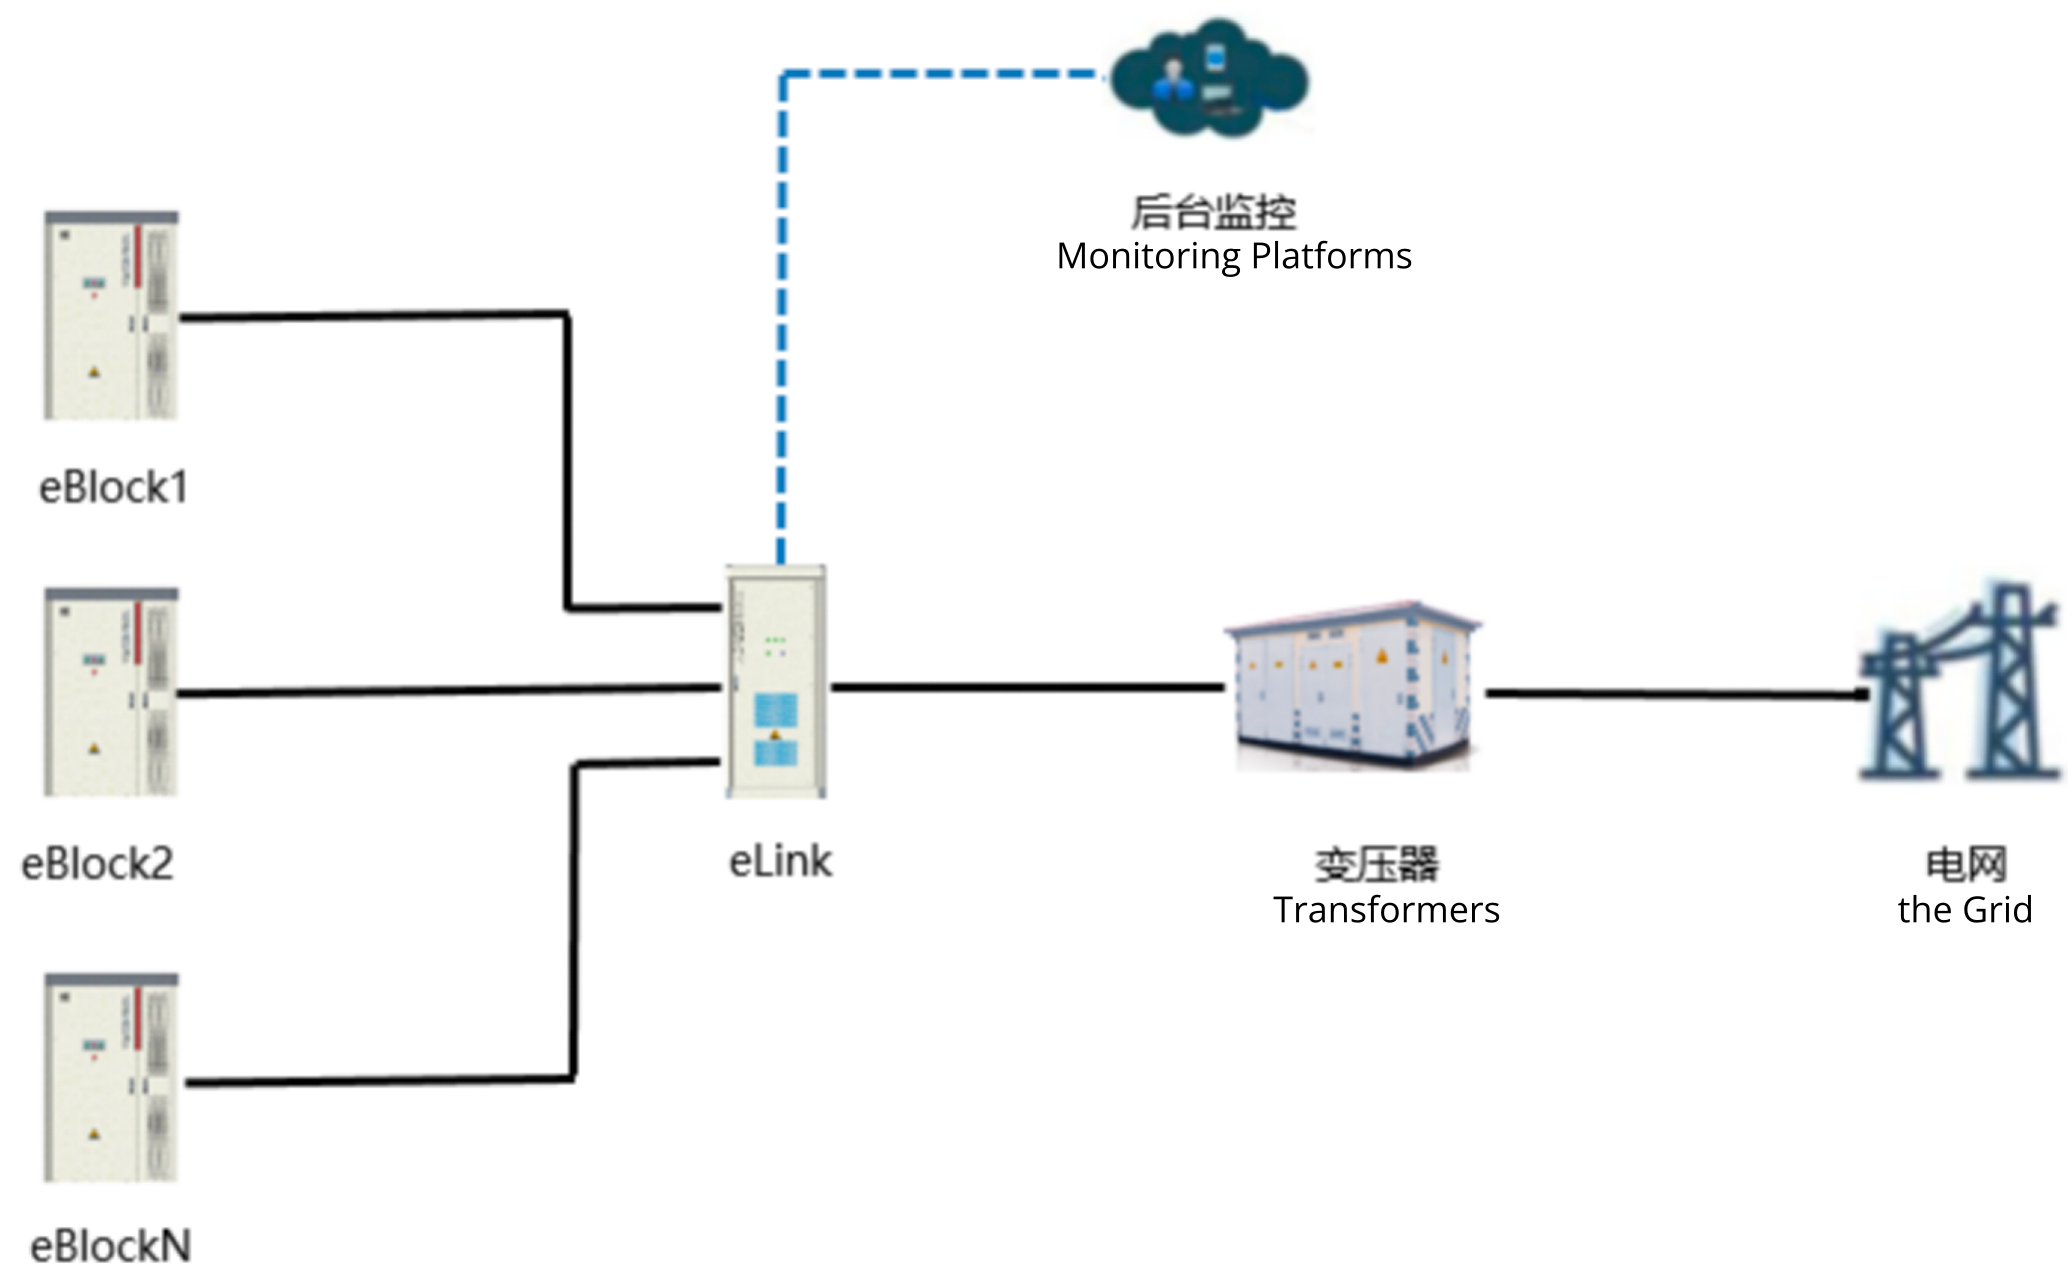
\includegraphics[width=0.8\textwidth]{topo_ess.png}
    \caption{Typical System Topology of eBlock--eLink Energy Storage Architecture}
\end{figure}


In discharge mode, the battery system converts \gls{dc} energy into grid-synchronized \gls{ac} power and feeds it to the grid. 

In charge mode, grid \gls{ac} power is converted into \gls{dc} power to charge the battery system.

\subsection{Introduction to eBlock}
The Smart Energy Block (eBlock) is an integrated device for energy storage and conversion in electrochemical energy storage systems. It can control the charging and discharging processes of batteries, perform \gls{ac}-\gls{dc} conversion, and directly supply power to \gls{ac} loads even in the absence of a grid. The Smart Energy Block (eBlock) consists of components such as battery modules (\gls{pack}), a \gls{pcs}, a cooling system, and cabinet structural parts.

\begin{figure}[htbp]
    \centering
    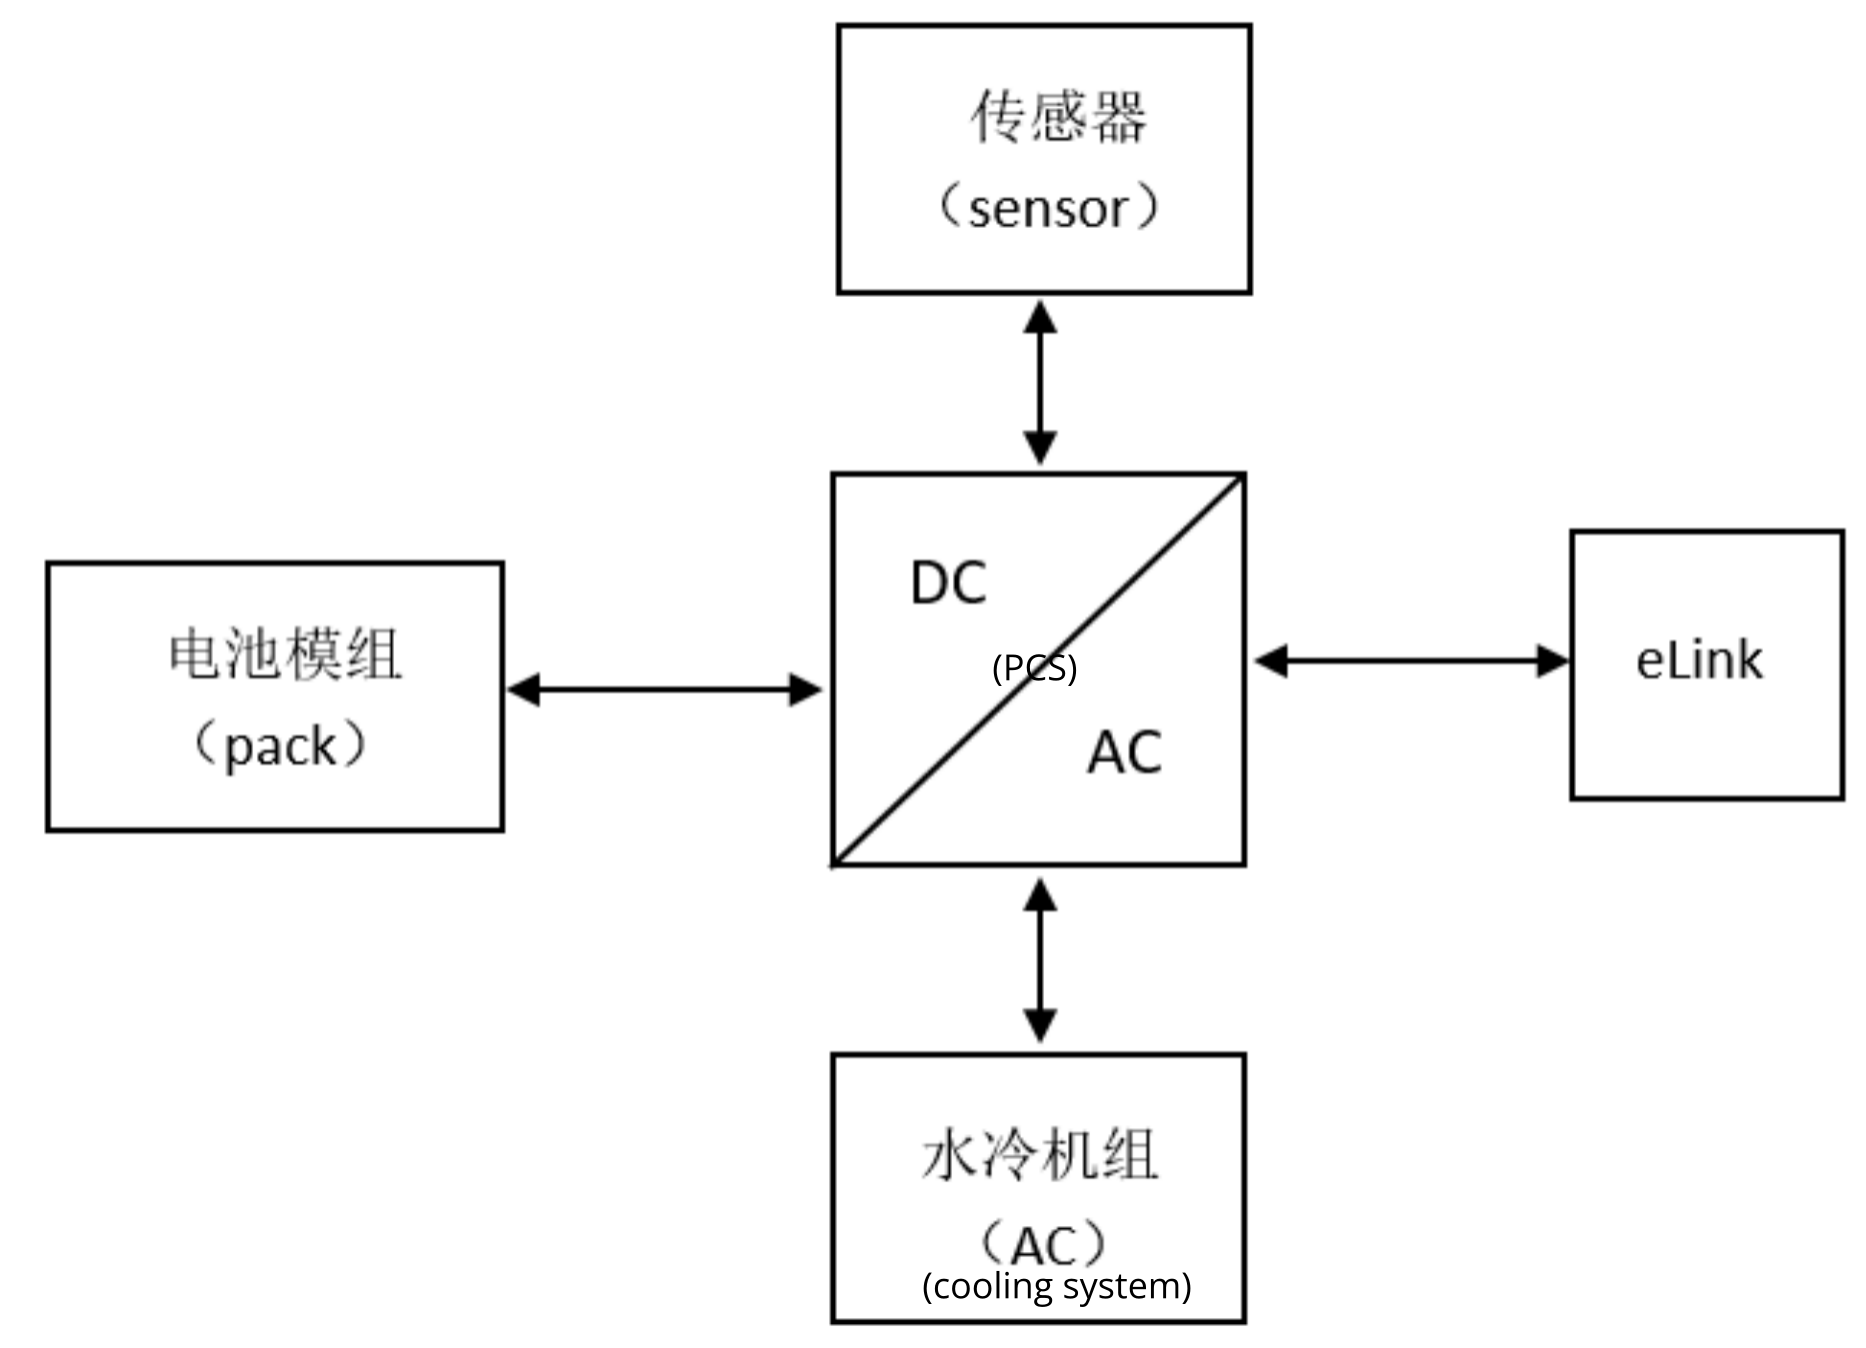
\includegraphics[width=0.8\textwidth]{topo_eblock.png}
    \caption{eBlock Architecture}
\end{figure}

% ==========================================
% Chapter 2: Personnel Entry Safety Precautions
% ==========================================
\section{Personnel Entry Safety Precautions}
\subsection{Personnel Qualification and Work Authorization}
\begin{itemize}[leftmargin=1.5em]
    \item Only trained and qualified electrical technicians are allowed to operate, open, move, wire, or maintain eBlock/eLink/PCS equipment.
    \item Battery-related maintenance shall be performed only by personnel with battery expertise and documented safety training.
    \item High-risk work (live verification, breaker isolation, internal cabinet access, and fire-system intervention) shall be executed under a permit-to-work or equivalent site authorization process.
    \item Maintenance tasks should be performed by at least two persons; single-person intervention is not recommended for energized or high-risk activities.
\end{itemize}

\subsection{Personal Protective Equipment (PPE), Tools, and Work Discipline}
\begin{itemize}[leftmargin=1.5em]
    \item Wear suitable PPE, including insulated gloves, insulated shoes, safety helmet, and eye protection.
    \item Remove rings, watches, and other conductive metal objects before approaching the equipment.
    \item Use only qualified insulated tools and calibrated test instruments suitable for the expected voltage level.
    \item Do not place tools or metal objects on top of cabinets, inside open compartments, or into internal cavities of the eBlock.
\end{itemize}

\subsection{Pre-entry and Site Safety Checks}
Before entering the operating area or opening cabinets, confirm the following:
\begin{itemize}[leftmargin=1.5em]
    \item Fire extinguishers and emergency access routes are available and unobstructed.
    \item The installation area is clean, dry, well ventilated, and free from standing water, corrosive gas, and combustible storage.
    \item Cabinet exteriors show no smoke, scorching, leakage, deformation, abnormal noise, or unusual odor.
    \item Real-time alarms on the \gls{hmi}, fire display, \gls{ups}, and controller are reviewed before work starts.
    \item Working scope, shutdown boundary, and emergency communication method are clearly understood by the on-site team.
\end{itemize}

\subsection{Electrical Isolation and Strict Prohibitions}
\begin{itemize}[leftmargin=1.5em]
    \item During wiring or maintenance, disconnect the AC switch/breaker before any operation.
    \item Do not touch internal electrical components before full shutdown, isolation, and discharge verification.
    \item Unauthorized personnel are strictly prohibited from opening the eBlock.
    \item Even without external power input, high voltage may still exist inside the equipment.
    \item Even when all switches and breakers are opened, hazardous voltage may remain in the eBlock; any opening or movement operation must be performed only by professional technicians.
    \item Keep equipment away from fire sources; do not install in flammable/explosive environments or near unprotected combustible hazards.
    \item Ensure all terminals and bolts are tightened properly to maintain reliable electrical contact under high-current operation.
\end{itemize}

% ==========================================
% Chapter 3: Installation Guide
% ==========================================
\section{Installation Guide}
\subsection{Integrated Installation Guide}
To achieve design performance and maximize service life, reserve sufficient installation and maintenance space, and execute all work strictly in accordance with approved drawings.

\subsection{Equipment Transportation and Storage}
\textbf{Transportation requirements}
\begin{itemize}[leftmargin=1.5em]
    \item Transportation/warehousing providers shall hold valid dangerous-goods qualifications in the project jurisdiction. Transport should be carried out using stake trucks to facilitate loading and unloading of equipment.
    \item Rough loading and unloading are strictly prohibited to prevent short-circuit, leakage, breakage, fire, or explosion.
    \item Before shipment, verify compliant declaration status and confirm packaging/labels are intact, with no odor, leakage, smoke, or ignition signs.
    \item Handle with care during loading, unloading and transportation. Packages shall be firmly secured, kept upright (no side placement or inversion), and protected against moisture during transport. Packaging should be securely tied to prevent displacement, and hazardous materials labels should face outwards.
\end{itemize}

\textbf{Storage requirements}
\begin{itemize}[leftmargin=1.5em]
    \item During storage, it is necessary to retain relevant documentation that meets the product's storage requirements, such as temperature and humidity log data, photos of the storage environment, and inspection reports.
    \item Store in a clean, dry place and protect from dust and moisture. Do not expose to rainwater or standing water on the ground.
    \item The ambient air must not contain corrosive or flammable gases.
    \item Do not store in a tilted or inverted position.
    \item Equipment other than battery packs, when stored for two years or longer, must undergo inspection and testing by qualified personnel before being put into use.
    \item The energy storage cabinet is recommended to be stored indoors, away from direct sunlight or rain, in a dry, well-ventilated area with a clean surrounding environment and free of any obstructions. Avoid exposure to intense infrared radiation and other types of radiation, as well as organic solvents, corrosive gases, and metallic conductive dust. Keep away from heat sources and ignition sources.
    \item When storing energy storage cabinets, please keep them separately and avoid mixing them with other equipment. The site must be equipped with fire-fighting facilities that meet the required standards, such as fire sand and fire extinguishers.
    \item It is recommended to use energy storage cabinets promptly. For energy storage cabinets stored for long periods, perform regular top-up charging; otherwise, it may cause damage to the energy storage cabinet.
\end{itemize}

\subsection{Installation Tools, Lifting, and Environment}
\textbf{Forklift and hoisting}
\begin{itemize}[leftmargin=1.5em]
    \item Recommended forklift capacity: \textbf{$\geq$ 5 t}; recommended fork length: \textbf{$\geq$ 1800 mm} with a width of 230–300 mm and a thickness of 25–80 mm.
    \item Forklift lifting height requirements: When the foundation height is {$\leq$ 0.3 m}, the lifting height must be \textbf{$\geq$ 2 m}; when the foundation height is > 0.3 m, the lifting height increases \textbf{accordingly}.
    \item Lifting hooks are commonly forged from high-quality carbon steel. After forging, they must undergo annealing treatment, with the requirement that their hardness reaches: \textbf{95 \textasciitilde 135 HB}. The surface of the hook shall be smooth and free from defects such as flaking, notches, sharp edges, or cracks. Weld repairs are prohibited for hooks that are worn or have cracks.
    \item When hooking the sling onto the hook, the sling should be hung down to the bottom of the hook. When directly hooking into the lifting eye of a component, avoid forcing or twisting the hook, as this could cause deformation of the hook or result in the sling slipping off the hook. 
    \item When installing and removing lifting equipment, do not drag it across the cabinet to prevent scratching the cabinet surface.
\end{itemize}

\textbf{Environmental conditions}
\begin{itemize}[leftmargin=1.5em]
    \item Installation ambient temperature should be within \textbf{-25\,$^{\circ}$C to 45\,$^{\circ}$C}.
    \item To extend the lifespan of the smart energy block, avoid direct sunlight exposure; a shaded installation location is a better choice.
    \item Maintenance clearance around the cabinet.
\end{itemize}

\subsection{Cable Installation and Electrical Connection}
\subsubsection{Preparation of Installation Tools}
The following tools are required for the routine maintenance and operation of the e-Block 250. \textbf{Note:} All handheld tools used for electrical work must be properly insulated.

\begin{tabularx}{\textwidth}{l l l X}
\toprule
\textbf{No.} & \textbf{Tool Name} & \textbf{Model/Spec} & \textbf{Purpose} \\
\midrule
1 & Phillips Screwdriver & M6 & Fastening screws \\
2 & Socket Wrench & 17\# & Securing AC cables \\
3 & Diagonal Pliers & -- & Cutting cable ties \\
4 & Wire Strippers & -- & Stripping cable insulation \\
5 & Utility Knife & -- & Unpacking and general use \\
6 & Wire Cutters & -- & Cutting cables \\
7 & Crimping Tool & -- & Terminating cable lugs \\
8 & Multimeter & $\ge$ 1500V DC & Testing ground connections and voltage \\
9 & Marker Pen & $\le$ 10mm dia. & Making alignment or status marks \\
10 & Steel Tape Measure & -- & Measuring distances \\
11 & Insulated Gloves & -- & Personal protection during operation \\
12 & Soldering Iron & 30W & Repairing communication cables \\
\bottomrule
\end{tabularx}

\subsubsection{Electrical Connection Requirements}
\begin{itemize}[leftmargin=1.5em]
    \item Execute electrical connection strictly according to approved schematics; cables/connectors shall be corrosion-resistant and flame-retardant.
    \item Ensure cable ampacity meets design requirements with engineering margin; terminations shall be mechanically secure and electrically reliable.
    \item The connection between the conductor and the terminal should not be subjected to any external forces other than the normal tensile force of the connection.
    \item When crimping wires to cold-pressed terminals, the crimping tool should be selected appropriately. The terminal crimping must be firm and reliable, with clearly visible crimp marks aligned along the axis of the wire and terminal, and without any damage to the core wire.
\end{itemize}

\subsubsection{Main power wiring}
Connect the cable from the branch circuit breaker of the eLink power cabinet to the lower U, V, and W terminals of the PCS on the eBlock side corresponding to the energy module, wiring in the order of Phase A, Phase B, and Phase C.

The PCS ground shall be shorted to the enclosure, with a wire gauge of \textbf{$\leq$ 6 mm$^2$}; the enclosure shall be reliably connected to the safety ground with a wire gauge of \textbf{$\leq$ 35 mm$^2$}.

The PCS, eLink power cabinet, transformer, and wiring must be connected according to phase sequence A, B, and C.

\begin{figure}[H]
    \centering
    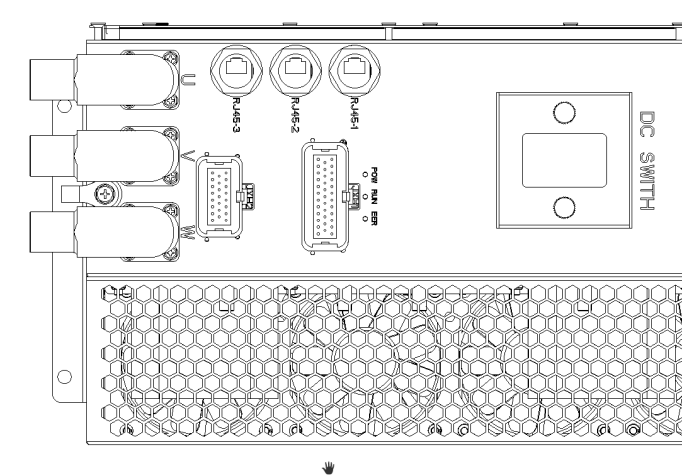
\includegraphics[width=0.8\textwidth]{3.1Schematic Diagram of AC Measurement Wiring Locations.png}
    \caption{Schematic Diagram of AC Measurement Wiring Locations}
\end{figure}

\begin{tabularx}{\textwidth}{l c}
\toprule
\textbf{Cable Type} & \textbf{Recommended cross-sectional area (mm$^2$)}\\
\midrule
AC cable with the 690V/1000V standard & 95 \\
\bottomrule
\end{tabularx}

\textbf{Note:} As far as possible, select multi-core armored cables for external cables to ensure a reliable connection of the smart power module.

\begin{figure}[H]
    \centering
    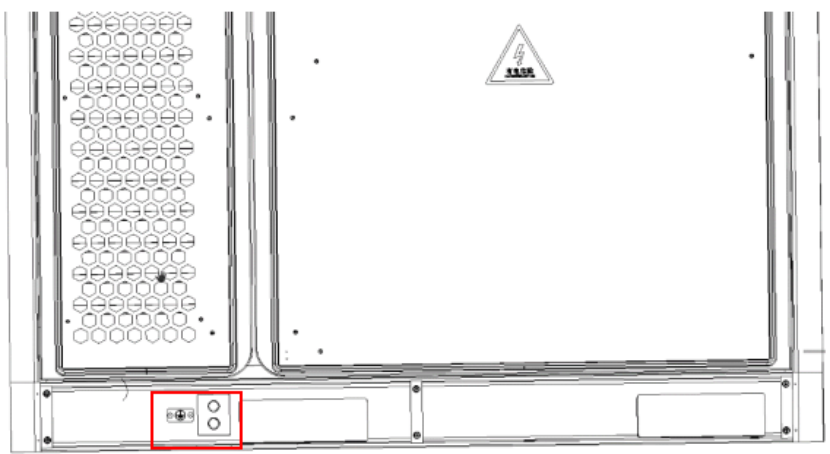
\includegraphics[width=0.8\textwidth]{3.2: Schematic Diagram of Grounding Locations.png}
    \caption{Schematic Diagram of Grounding Locations}
\end{figure}

{\renewcommand\tabularxcolumn[1]{m{#1}}
\begin{tabularx}{\textwidth}{>{\centering\arraybackslash}m{0.16\textwidth} >{\raggedright\arraybackslash}m{0.18\textwidth} >{\raggedright\arraybackslash}X}
\toprule

\includegraphics[height=3.2em]{warning.png} & \symname{Warning} & \symdesc{The protective grounding wire must be connected correctly; otherwise, the equipment will be damaged.} \\
\bottomrule
\end{tabularx}
}

In energy storage systems, all non-current-carrying metal components and equipment enclosures should be connected to earth (PE), M10 Screw tightening force 16.4N/m. The recommended diameter of the grounding wire (yellow-green, copper wire) is as shown in the table:

\begin{tabularx}{\textwidth}{c c c}
\toprule
\textbf{Recommended wire diameter (mm)} & \textbf{Cross-sectional area (mm$^2$)} & \textbf{Color}\\
\midrule
5.0\textasciitilde10.0 & 50 mm$^2$ & Yellow-Green\\
\bottomrule
\end{tabularx}

\textbf{Note:} The ground wire diameter shall not be \textbf{$\leq$ 35 mm$^2$}.

\subsubsection{Install the auxiliary power supply cable for the cabinet}
Connect a cable from the circuit breaker on the auxiliary power side of the eLink control cabinet to the junction box on the PCS side of the corresponding energy block eBlock. Then, run a cable from the junction box to the AC 230V terminal on the upper part of the PCS.

Connect a cable from the circuit breaker on the auxiliary power side of the eLink control cabinet to the junction box located beneath the water-cooling unit on the eBlock side. Then, run another cable from the junction box to the AC 220V power supply at the lower end of the water-cooling unit.

\begin{figure}[H]
    \centering
    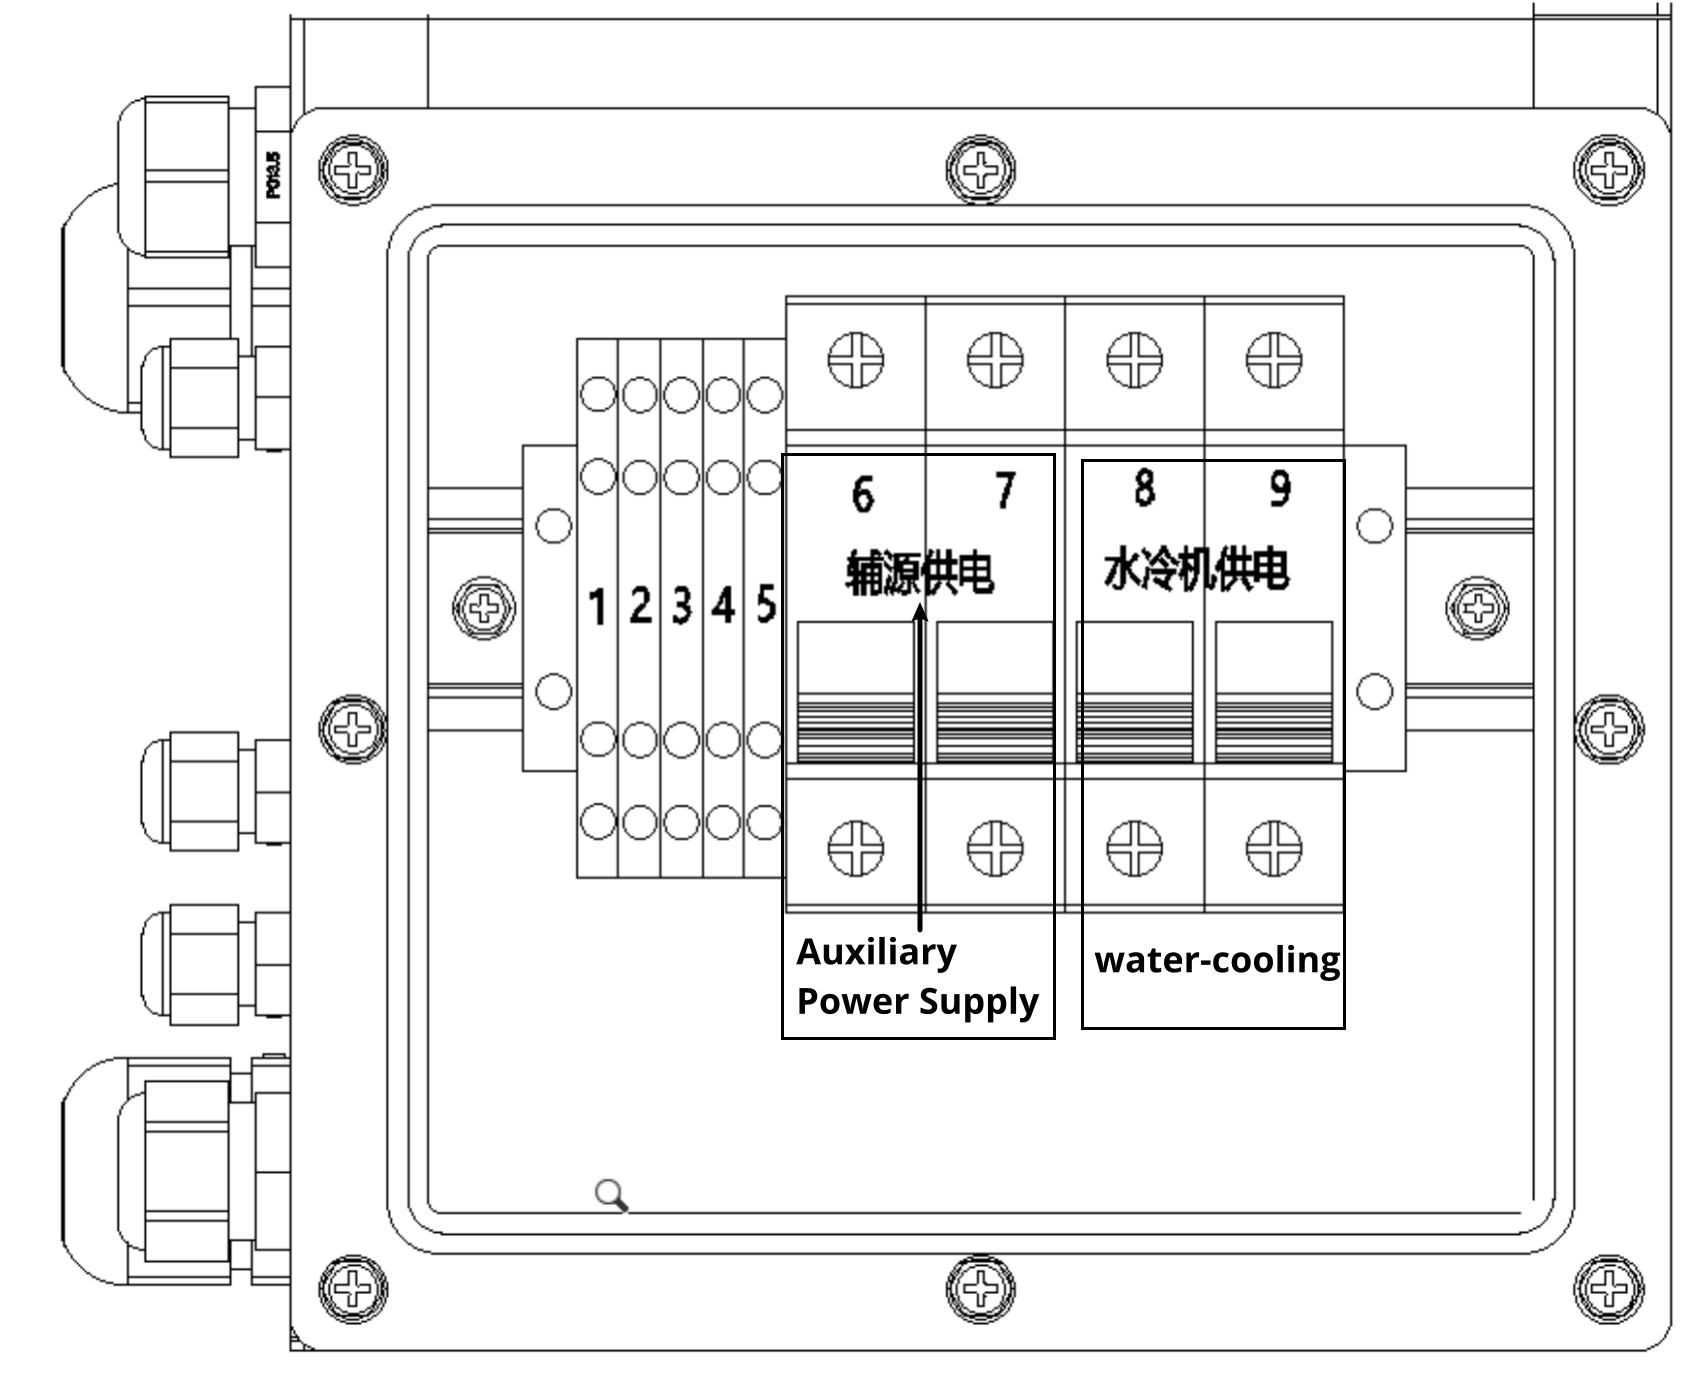
\includegraphics[width=0.8\textwidth]{3.3: Schematic Diagram of Auxiliary Power Supply Connection Location.png}
    \caption{Schematic Diagram of Auxiliary Power Supply Connection Location}
\end{figure}

The port wiring is shown in the table below:

\begin{tabularx}{\textwidth}{l l X} % 将最后一列改为 X
\toprule
\textbf{No.} & \textbf{Port Definition} & \textbf{Recommended Cross-section (mm$^2$)} \\
\midrule
3 & Parallel machine CAN\_H & 0.5 \\ % 注意：下划线 _ 需要加反斜杠 \_
4 & Parallel machine CAN\_L & 0.5 \\
5 & GND & 0.5 \\
6 & Auxiliary power supply L phase & 1 \\
7 & Auxiliary power supply N phase & 1 \\
8 & Water-cooled unit power supply L phase & 6 \\
9 & Water-cooled unit power supply N phase & 6 \\
\bottomrule
\end{tabularx}

\subsubsection{Install the cabinet communication cable}
Connect a network cable from the 24-port industrial switch in the eLink control cabinet to the RJ45-3 port on the PCS side of the corresponding energy block eBlock, and tighten the knob.

\begin{figure}[H]
    \centering
    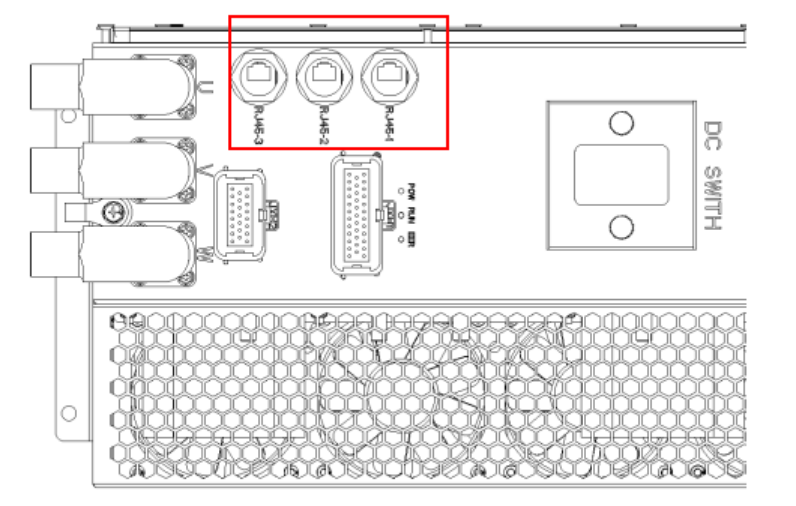
\includegraphics[width=0.8\textwidth]{3.4Communication Connection Location.png}
    \caption{Communication Connection Location}
\end{figure}

{\renewcommand\tabularxcolumn[1]{m{#1}}
\begin{tabularx}{\textwidth}{>{\centering\arraybackslash}m{0.16\textwidth} >{\raggedright\arraybackslash}m{0.18\textwidth} >{\raggedright\arraybackslash}X}
\toprule

\includegraphics[height=3.2em]{attention.png} & \symname{Attention} & \symdesc{The LAN communication cable is shielded twisted pair. The network cable length cannot exceed 90m, recommended $\leq$ 30m.} \\
\bottomrule
\end{tabularx}
}

\subsection{Safety Compliance Tests Before Commissioning}
Before safety tests, ensure the eBlock AC breaker is open, PCS AC220V auxiliary control power is not connected, primary wiring is tightened, and MSD status is correct.

% --- 方案：通过修改列定义实现顶部对齐 ---
\begin{tabularx}{\textwidth}{>{\sffont\raggedright\arraybackslash}p{2.5cm} X X} 
\toprule
\textbf{Test Item} & \textbf{Test Procedure} & \textbf{Acceptance Criteria} \\
\midrule
Insulation Resistance & Connect the positive clip to the +/- DC bus and the negative clip to the cabinet. & At 2500VDC for 60s, insulation resistance shall be \textbf{$\ge$ 10 M$\Omega$}. \\
\addlinespace
Withstand Voltage & In the withstand voltage interface. Test the PCS DC side and PACK total positive/negative to ground. & At 3820VDC for 60s, no breakdown, sparking, or flashover. PCS leakage $\le$ 10mA, PACK leakage $\le$ 1mA. \\
\addlinespace
Ground Continuity & Connect one end of the tester to the PCS ground and the other to the eBlock door ground. & Test current 30A for 60s, measured resistance \textbf{$\le$ 0.1 $\Omega$}. \\
\bottomrule
\end{tabularx}

{\renewcommand\tabularxcolumn[1]{m{#1}}
\begin{tabularx}{\textwidth}{>{\centering\arraybackslash}m{0.16\textwidth} >{\raggedright\arraybackslash}m{0.18\textwidth} >{\raggedright\arraybackslash}X}
\toprule

\includegraphics[height=3.2em]{attention.png} & \symname{Attention} & \symdesc{Short-circuit testing between positive and negative poles is strictly prohibited.} \\
\bottomrule
\end{tabularx}
}

% ==========================================
% Chapter 6: Maintenance and Care
% ==========================================
\section{Maintenance and Care}

\subsection{Daily Maintenance}
\textbf{Visual inspection}
\begin{itemize}[leftmargin=1.5em]
    \item Check cabinet exterior for water ingress, dents, paint damage, corrosion, deformation, smoke marks, and abnormal odor.
    \item Check whether the air filters at inlet/outlet of eLink and fire-cabinet air conditioners are blocked.
    \item Open the eBlock cabinet and check coolant level and pressure (for units equipped with sight glass and pressure gauge).
    \item Inspect PCS appearance for bulging/deformation; confirm PCS inlet/outlet filters are free of heavy dust and blockage.
    \item Inspect PACK condition: no swelling, leakage, deformation, or damage; verify cable terminals are secure and free of burning/melting traces.
    \item Check eLink power cabinet for arc-blackening traces, abnormal noise/vibration/smoke, water ingress, and odor.
    \item Check eLink control cabinet status: normal HMI display, no unexplained alarms, normal UPS output, no breaker trip, normal switch link lights, and normal cabinet AC operation.
    \item Check fire-control display indicators, including host battery level, display-controller battery level, and liquid level.
\end{itemize}

\textbf{Operational and environmental checks}
\begin{itemize}[leftmargin=1.5em]
    \item Connect a service computer to the eLink device-layer switch and perform one-click parameter readback; verify no abnormal configuration.
    \item Inspect environmental conditions and filter blockage status for PCS, cabinet AC units, and water-cooling units.
    \item Check all relay devices on the fire-control screen; verify host battery, display-controller battery, and liquid-level indicators are within normal range.
\end{itemize}

{\renewcommand\tabularxcolumn[1]{m{#1}}
\begin{tabularx}{\textwidth}{>{\centering\arraybackslash}m{0.16\textwidth} >{\raggedright\arraybackslash}m{0.18\textwidth} >{\raggedright\arraybackslash}X}
\toprule

\includegraphics[height=3.2em]{attention.png} & \symname{Attention} & \symdesc{When performing maintenance tasks such as system cleaning, electrical connections, and ensuring reliable grounding, first disconnect the circuit breaker connected to the AC side of the grid, then disconnect the DC-side circuit breaker inside the smart energy module. After power is cut off, please wait at least \textbf{30 minutes}, then proceed with the operation.} \\
\bottomrule
\end{tabularx}
}

\subsection{Regular Maintenance}
\begin{tabularx}{\textwidth}{>{\sffont\raggedright\arraybackslash}p{4cm} >{\hsize=1.4\hsize\raggedright\arraybackslash}X >{\hsize=0.6\hsize\raggedright\arraybackslash}X}
\toprule
Item & Method / Criteria & Interval \\
\midrule
System cleaning & Inspect inlets/outlets for blockage and dust contamination; clean regularly. & Every 6--12 months \\
Operating status & Check cabinet appearance, listen for abnormal sound, and verify operating parameters. & Every 6 months \\
Electrical connection & Check cable terminals for loosening/detachment and insulation damage at metal contact points. & First at 6 months, every 6--12 months \\
Grounding reliability & Verify all grounding conductors are securely and reliably bonded. & First at 6 months, every 6--12 months \\
Fire modules & Inspect monitoring/alarm/protection modules and terminal harnesses; replace damaged parts promptly. & Weekly / outage inspection \\
Cooling unit & Verify voltage/current/inlet-outlet temperature/pressure/operating sound. & Routine \\
\bottomrule
\end{tabularx}

\subsection{Daily Maintenance of Firefighting Equipment}
\begin{itemize}[leftmargin=1.5em]
    \item Weekly check: inspect all terminal and harness connections; verify monitoring and alarm modules are operational; visually check for external damage or missing parts.
    \item Outage inspection: inspect monitoring, alarm, and protection modules for cracks, dents, deformation, corrosion, and missing parts; replace damaged components promptly.
\end{itemize}

\subsection{Daily Maintenance of Water-Cooled Units}
Routine maintenance is preventive maintenance aimed at identifying alarms/fault risks early and ensuring long-term stable operation.
\begin{itemize}[leftmargin=1.5em]
    \item Detect and handle early alarms before they escalate.
    \item Eliminate fault risks in early stage to avoid economic loss and service interruption.
    \item Analyze operating trends and implement targeted optimization.
\end{itemize}

\subsection{Maintenance and Inspection Schedule}
Regular inspection of the cooling unit is essential for system reliability. Follow the standards and methods defined in the table below:

% 使用带有自适应换行的顶部对齐排版
\begin{tabularx}{\textwidth}{>{\sffont\raggedright\arraybackslash}p{2.2cm} >{\raggedright\arraybackslash}p{5.2cm} >{\raggedright\arraybackslash}p{4cm} X}
\toprule
\textbf{Maintenance Item} & \textbf{Maintenance Standards} & \textbf{Detection Method} & \textbf{Exception Handling} \\
\midrule
Running Data & 
Current: $<$ Max on nameplate.\par
Voltage: AC 220V $\pm$10\%.\par
Inlet Temp: 12$^\circ$C--37$^\circ$C.\par
Outlet Temp: 10$^\circ$C--37$^\circ$C. & 
Monitor via HMI "Ring" or "Environment State" interface. & 
Contact JDEnergy support. \\
\addlinespace

Running Sound & 
The unit operates without abnormal vibrations or noise. & 
Auditory check of: Compressor, Fan, and Circulating pump. & 
Contact JDEnergy support. \\
\addlinespace

Pipeline \newline Reliability & 
\textbf{Refrigerant:} No leaks. \par High-pressure: 7.0--27.0 bar. \par Low-pressure: 0.5--4.0 bar.\par
\textbf{Coolant:} No leaks. \par Static: 0.8--1 bar. \par Operating: 0.8--1.9 bar. & 
Visual inspection and pressure gauge reading. & 
Contact JDEnergy support. \\
\addlinespace

Unit \newline Exterior & 
The unit's surface is clean, dust-free, and free of dirt. & 
Visual inspection. & 
Clean by a brush or cotton cloth. \\
\bottomrule
\end{tabularx}

\subsection{Coolant Refilling Procedure (Water-Cooling Unit)}
\textbf{Pre-checks}
\begin{itemize}[leftmargin=1.5em]
    \item Device Connection: Connect the water machine's external display to the “communication port.” (When the handheld operator screen is connected to the screen plug, the water machine's communication system will prioritize receiving signals from the communication port. Therefore, after unplugging the communication port plug, insert the water machine's handheld operator screen into the communication port.)
    \item Pipe Connection: Remove the plug from the upper exhaust valve, and insert the drain pipe into the exhaust valve. (During the refilling process, if air is not being purged, the exhaust pipe must be plugged to prevent coolant from leaking out.)
    \item Pump Connection: Use a qualified make-up water pump. The inlet must be equipped with a check valve to prevent fluid backflow, and the outlet must have a quick-connect fitting for connection to the liquid-cooling unit's fill port.
\end{itemize}

\begin{figure}[H]
    \centering
    % 第一张子图
    \begin{minipage}[t]{0.48\textwidth}
        \centering
        % 设定统一的高度，例如 6cm，keepaspectratio 确保图片不失真
        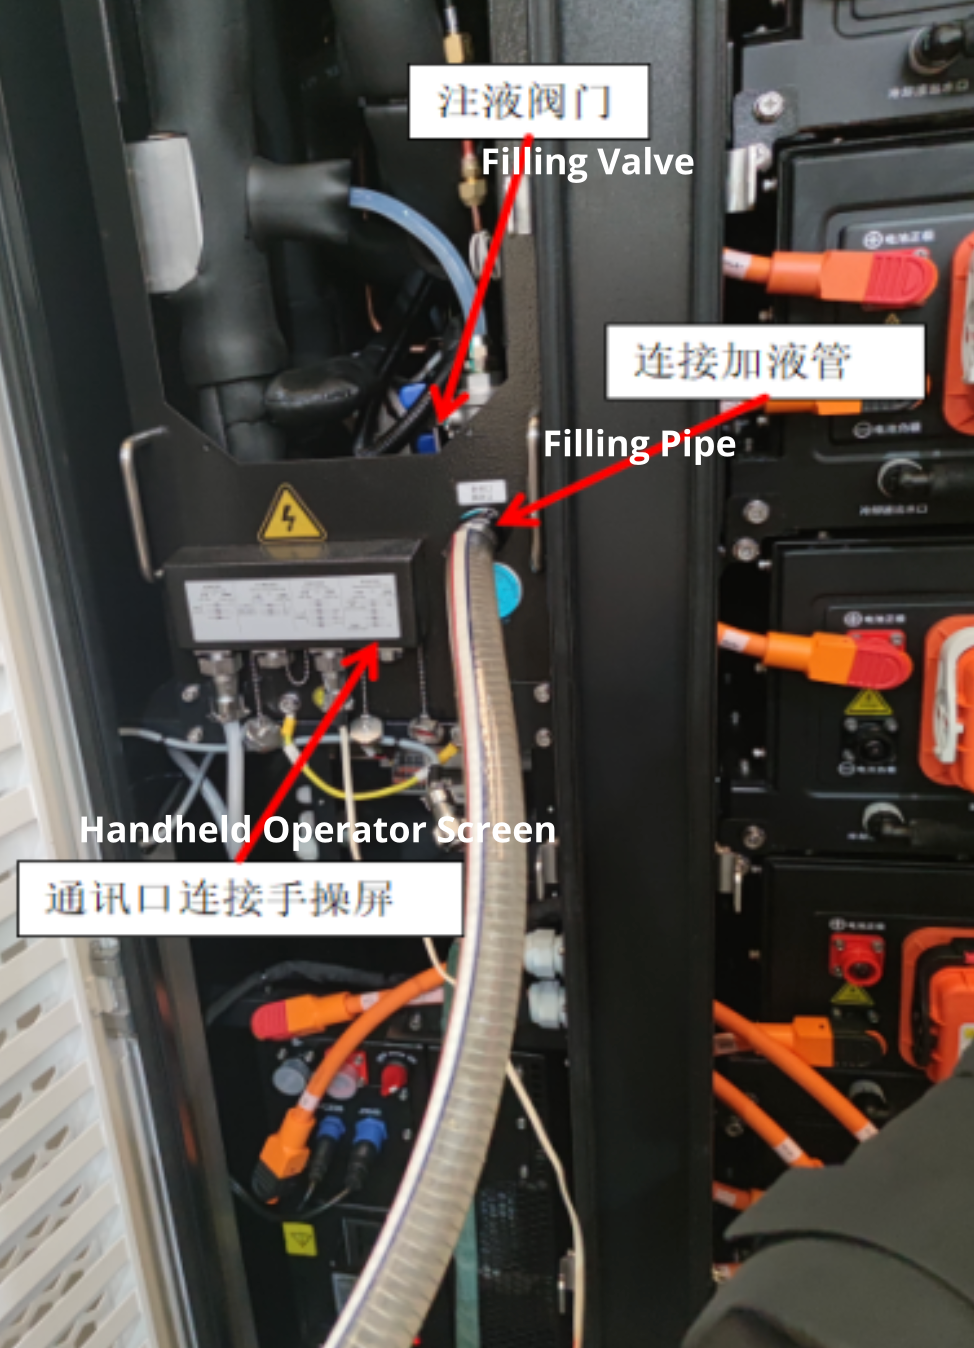
\includegraphics[height=6cm, width=2\textwidth, keepaspectratio]{4.1Pipe Installation.png}
        \caption{Pipe Installation}
    \end{minipage}
    \hfill 
    % 第二张子图
    \begin{minipage}[t]{0.48\textwidth}
        \centering
        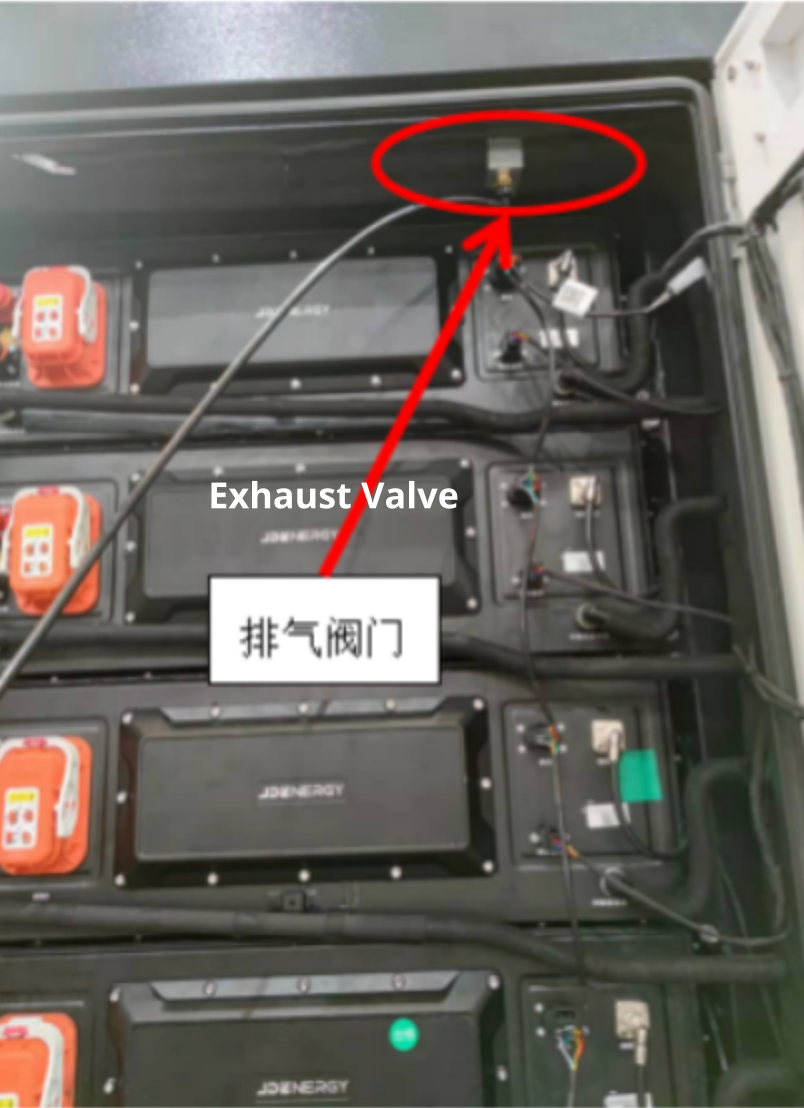
\includegraphics[height=6cm, width=2\textwidth, keepaspectratio]{4.2Exhaust Pipe Installation.png}
        \caption{Exhaust Pipe Installation}
        \label{fig:exhaust_install}
    \end{minipage}
\end{figure}

\textbf{Liquid addition step}
\begin{itemize}[leftmargin=1.5em]
    \item Remove the four screws securing the chiller's outer cover, and close the filling valve located behind the drain port.
    \item As shown in Figures \ref{fig:exhaust_install}, connect the vacuum pump to the exhaust valve located above the water-cooling pipeline using a connecting tube. Before operation, ensure that the connecting tubing is completely free of water or any other liquid.
    \item Tap the power button on the touch screen to start the water-cooling unit. Tap the “magnifying glass” button to enter the parameter interface. If an alarm occurs, tap the alarm icon and then tap “Clear Alarm.”
    \item The fluid infusion pump is connected at one end to the injection port of the chiller, and its inlet port is connected to the liquid storage tank. If there is air in the connecting tubing, purge the air from the tubing before injecting the fluid.
    \item Open the injection valve and turn on the replenishment pump switch to perform the injection operation.
    \item Observe the water supply and return pressure on the hand-operated screen. Stop adding fluid when the supply pressure stabilizes at 1.5–1.6 bar.
\end{itemize}

\textbf{Liquid injection finishing}
\begin{itemize}[leftmargin=1.5em]
    \item Unplug the handheld screen and reinsert the original communication cable into the communication port.
    \item When removing the quick connector from the filling port, be aware that some antifreeze residue remains in the water-cooling unit—from the filling valve all the way to the filling port—and should be collected using a container. A small amount of coolant may leak out; promptly wipe it up with a dry cloth or dry paper towel to prevent splashing, and then securely replace the dust cap on the filling port.
    \item After the liquid injection is complete, replace the corresponding dust caps, and check the status of the unit valves again.
\end{itemize}

\subsection{Wear Part Management}
Maintain a controlled spare-parts inventory for high-consumption and critical components, including (as applicable): 

\begin{tabularx}{\textwidth}{>{\sffont\raggedright\arraybackslash}p{5cm} X}
\toprule
\textbf{Name} & \textbf{Specifications} \\
\midrule
Network Controller IO & CX-5216E-QD \\
\addlinespace
Circuit breaker & Miniature circuit breaker / 240V / 32A / 1P \\
\addlinespace
Energy storage converter & PCS-2000 / PCS-2000G2 \\
\addlinespace
Network I/O Controller & Ethernet Remote Controller (16 DI, 16 Relay Outputs, 1 RS232 Port, 1 RS485 Port) \\
\addlinespace
PCBA Three-Proofing & BMUP52 Serial Motherboard / Three-Proofing \\
\addlinespace
Circuit breaker & Molded-case circuit breaker / 690V AC / 250A / 3P / with auxiliary contacts \\
\addlinespace
UPS & YTR1102L \\
\addlinespace
Display screen & 710.1-inch LCD 1024*600 touch screen \\
\addlinespace
Device Management Machine & eLink-2000 \\
\bottomrule
\end{tabularx}

\subsection{Maintenance Precautions}
\begin{itemize}[leftmargin=1.5em]
    \item Safety first: work in pairs and never perform high-risk maintenance alone.
    \item Maintenance shall be performed by qualified or manufacturer-trained personnel only.
    \item Record maintenance data, findings, and corrective actions in the service report.
\end{itemize}

\subsection{Inspection Checklist Reference}
Detailed inspection and patrol forms are provided in the appendices and should be used as controlled O\&M records.

% ==========================================
% Chapter 7: Safety Precautions
% ==========================================
\section{Safety Precautions}

\subsection{Operational Safety}
\begin{itemize}[leftmargin=1.5em]
    \item The energy storage cabinet is high-voltage equipment; unauthorized contact with internal electrical components is strictly prohibited.
    \item Non-professional personnel shall keep a safe distance when approaching energized equipment.
    \item If leakage, sparking, smoke, or abnormal odor is detected, stop operation immediately, isolate power with insulated tools, and notify qualified personnel.
    \item Install and operate cabinets in fire-compliant locations with suitable extinguishers (CO$_2$ / dry powder) available.
    \item Keep surroundings clean; do not store flammable or explosive materials near the cabinet; keep fire passages unobstructed.
    \item Ensure adequate ventilation during operation and respond immediately to overheating indications.
    \item Do not place objects on the cabinet; avoid severe vibration or impact during operation.
    \item The energy storage cabinet is intended solely for storing and managing electrical energy; it is strictly prohibited to use it for any other purposes not specified in its design.
\end{itemize}

\subsection{Maintenance Safety}
\begin{itemize}[leftmargin=1.5em]
    \item Before maintenance, disconnect power according to procedure and verify complete discharge status on HMI or with approved discharge equipment.
    \item Wear qualified PPE: insulated gloves, insulated shoes, safety helmet, and safety goggles.
    \item Use only insulated and qualified tools; follow approved disassembly/assembly procedures.
    \item For testing and measurement, use calibrated professional instruments and follow instrument operating instructions.
\end{itemize}

\subsection{Equipment Power-off Operation}
\label{subsec:equipment-power-off}

To ensure the safety of personnel and equipment, the power-off operation must follow the specific sequences defined below.

% --- 流程 1: eBlockPCS ---
\subsubsection*{A. Power-off Sequence for eBlockPCS}
\begin{figure}[H]
    \centering
    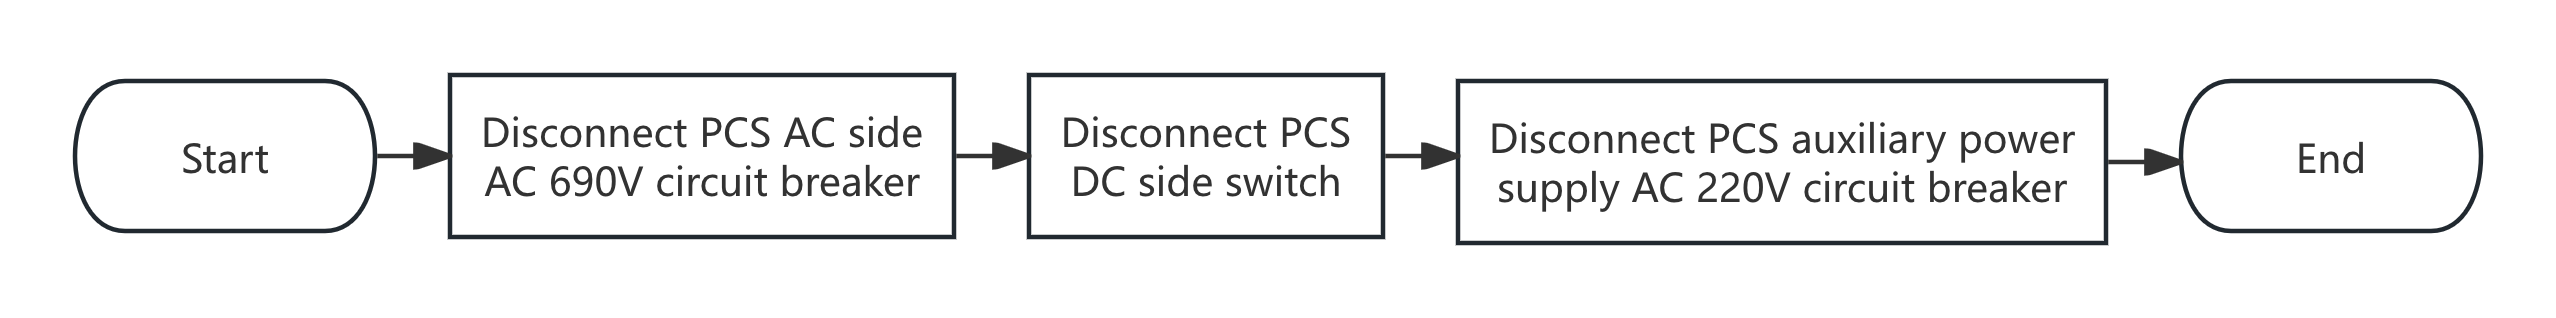
\includegraphics[width=1.5\textwidth]{5.1Power-off Sequence for eBlockPCS.png}
    \caption{Power-off Sequence for eBlockPCS}
\end{figure}

% --- 流程 2: eBlock ---
\subsubsection*{B. eBlock Power-Off Sequence}
\begin{figure}[H]
    \centering
    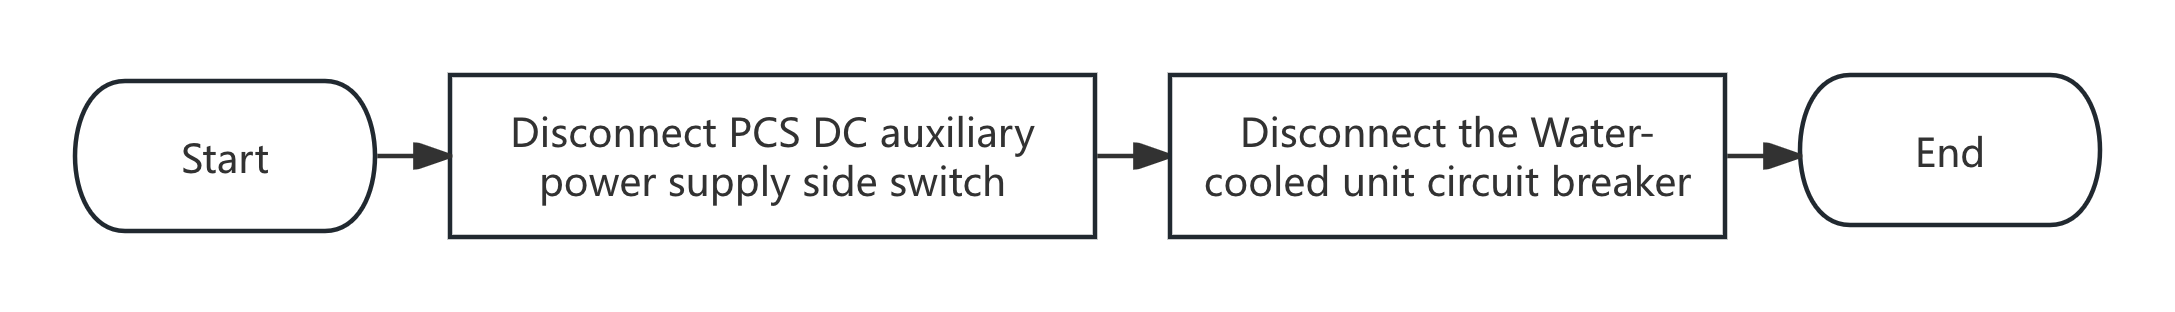
\includegraphics[width=\textwidth]{5.2eBlock Power-Off Sequence.png}
    \caption{eBlock Power-Off Sequence}
\end{figure}

% --- 流程 3: ESS Fire Suppression ---
\subsubsection*{C. Power-off Sequence for Energy Storage Fire Suppression System}
\begin{figure}[H]
    \centering
    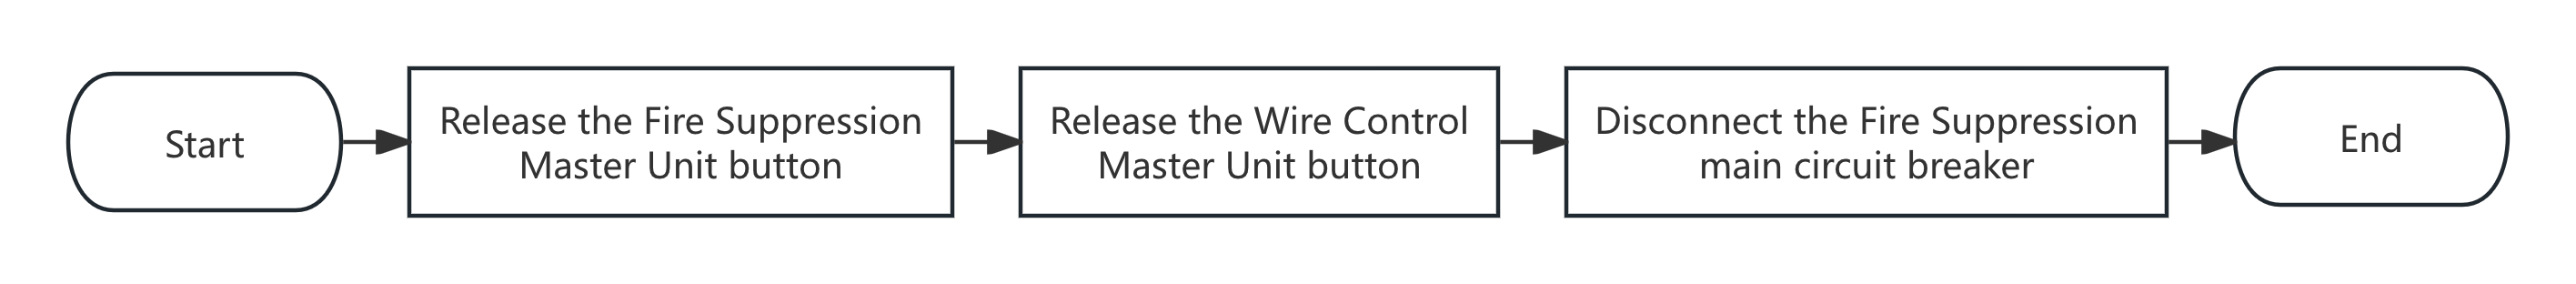
\includegraphics[width=\textwidth]{5.3Power-off Sequence for Energy Storage Fire Suppression System.png}
    \caption{Power-off Sequence for Energy Storage Fire Suppression System}
\end{figure}

\subsection{Equipment Energization Operation}

The energization process must be carried out in a strict sequence to prevent inrush current damage and ensure system stability.

% --- 流程 1: eBlockPCS ---
\subsubsection*{A. eBlockPCS Power-On Sequence}
\begin{figure}[H]
    \centering
    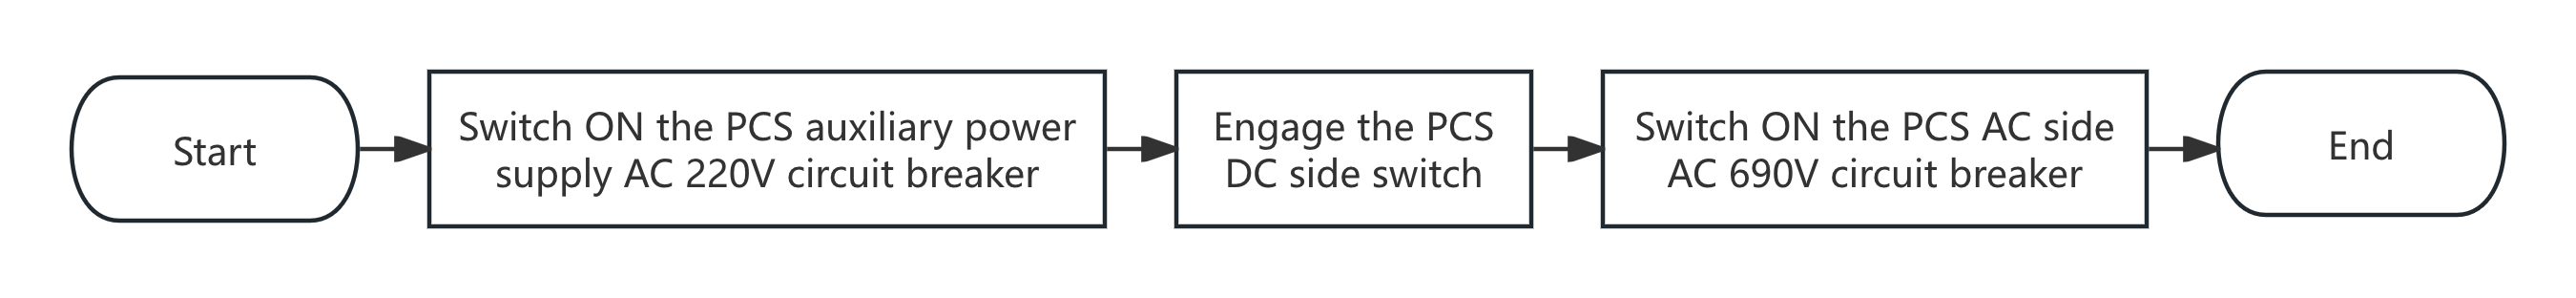
\includegraphics[width=\textwidth]{5.4eBlockPCS Power-On Sequence.png}
    \caption{eBlockPCS Power-On Sequence}
\end{figure}

% --- 流程 2: eBlock ---
\subsubsection*{B. eBlock Power-On Sequence}
\begin{figure}[H]
    \centering
    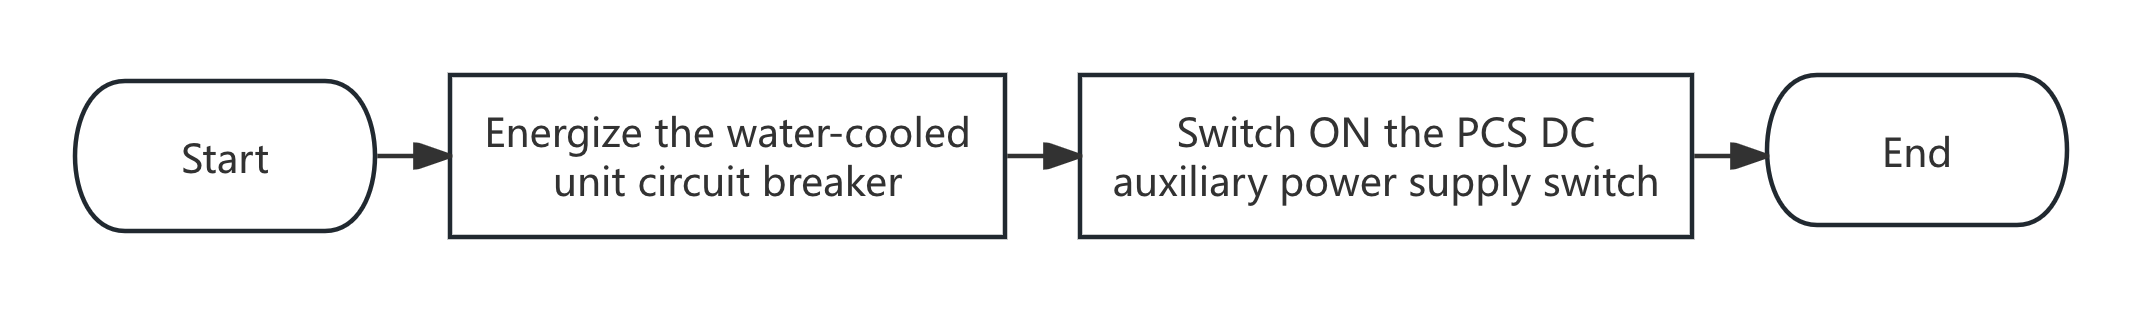
\includegraphics[width=\textwidth]{5.5eBlock Power-On Sequence.png}
    \caption{eBlock Power-On Sequence}
\end{figure}

% --- 流程 3: Fire Protection ---
\subsubsection*{C. Sequence of Power Supply for Energy Storage Fire Protection}
\begin{figure}[H]
    \centering
    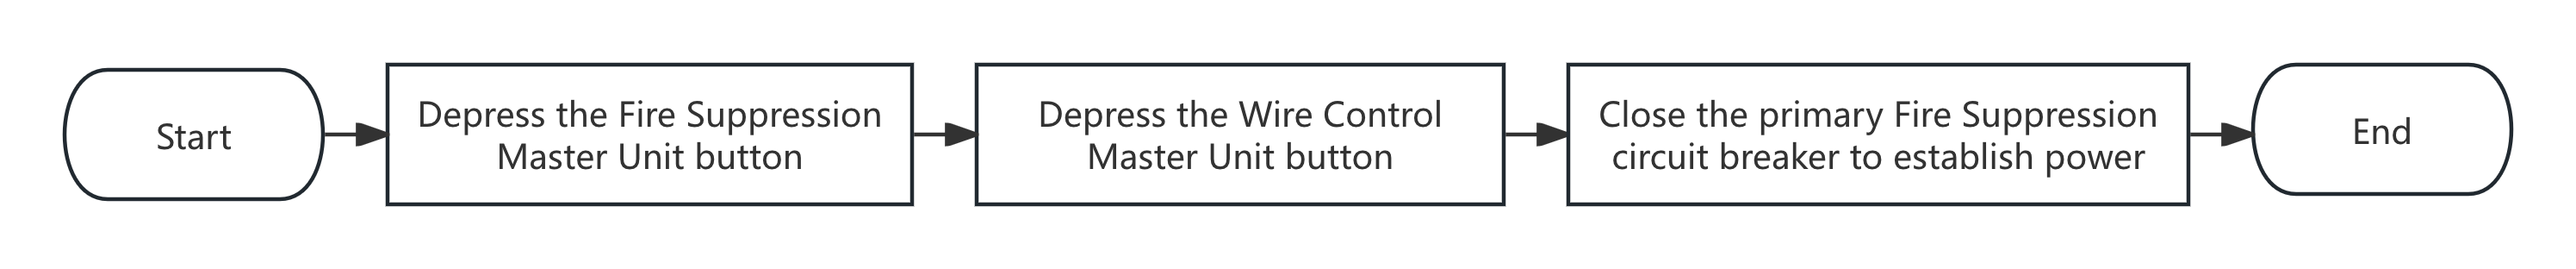
\includegraphics[width=\textwidth]{5.6Sequence of Power Supply for Energy Storage Fire Protection.png}
    \caption{Sequence of Power Supply for Energy Storage Fire Protection}
\end{figure}

% ==========================================
% Chapter 8: Troubleshooting
% ==========================================
\section{Troubleshooting}

\subsection{Common Fault Symptoms, Causes, and Actions}
The following table provides a guide for identifying and resolving common system malfunctions. If a fault persists after performing the suggested actions, please contact technical support.

% 设置跨页表格
\begin{xltabular}{\textwidth}{>{\sffont\raggedright\arraybackslash}X >{\raggedright\arraybackslash}X >{\raggedright\arraybackslash}X}
\toprule
\textbf{Malfunction} & \textbf{Possible Causes} & \textbf{Solution} \\
\midrule
\endfirsthead % 第一页页头

\toprule
\textbf{Malfunction} & \textbf{Possible Causes} & \textbf{Solution} \\
\midrule
\endhead % 后续页面的重复页头

\midrule
\multicolumn{3}{r}{Continued on next page...} \\
\endfoot % 页脚提示

\bottomrule
\endlastfoot % 最后一页的底部线

% --- 表格内容开始 ---
Equipment shutdown & PCS alarm or fault. & Contact the manufacturer's after-sales service. \\ \addlinespace
Charging abnormality & PCS failure. & Replace the PCS unit. \\ \addlinespace
Discharge abnormality & PCS failure. & Replace the PCS unit. \\ \addlinespace
BCS shutdown & Caused by a BCS failure. & Contact the manufacturer's after-sales service for specific fault inquiries. \\ \addlinespace
DC bus connection fault & PCS DC contactor failure. & Replace the PCS unit. \\ \addlinespace
BMU communication failure & Sampling harness loose or \gls{bmu} board faulty. & Retighten the BMU communication harness or replace the BMU acquisition board. \\ \addlinespace
Alarm light flashing & Door latch malfunction or door not closed tightly. & Replace the door magnetic switch or ensure the door is closed securely. \\ \addlinespace
Meter communication failure & Incorrect RS485 wiring or meter malfunction. & Contact the manufacturer's after-sales service. \\ \addlinespace
PCS soft-start failure & Internal system error. & Power off and restart, or replace the PCS. \\ \addlinespace
PCS bus voltage low & Internal system error. & Power off and restart, or replace the PCS. \\ \addlinespace
PCS overcurrent & Internal system error. & Power off and restart, or replace the PCS. \\ \addlinespace
Water-cooled AC malfunction & Low pressure in unit or water machine malfunction. & Top up the coolant or contact the manufacturer's after-sales service. \\ \addlinespace
Battery charging overvoltage & Sampling anomaly or harness fault. & Power off and restart, or replace the voltage and temperature sampling harness. \\ \addlinespace
Battery discharge undervoltage & Sampling anomaly or harness fault. & Power off and restart, or replace the sampling harness and recharge cells. \\ \addlinespace
Low-temperature battery & AC malfunction or temperature sampling harness failure. & Contact the manufacturer's after-sales service. \\ \addlinespace
Temperature abnormality alarm & Case temperature too high (ambient or blocked vents). & Check ambient temperature and ensure ventilation holes are not blocked. \\ \addlinespace
Circuit breaker trips repeatedly & Circuit protection or short circuit. & Identify the short-circuit point before resetting. If not found, contact the manufacturer. \\ \addlinespace
Lightning protection failure & Surge protector (\gls{spd}) is damaged. & Replace the AC surge protector board. \\ \addlinespace
Grid voltage abnormality & Grid voltage higher or lower than standard limits. & Check the power grid or contact the manufacturer. \\ \addlinespace
Grid frequency abnormality & Grid frequency out of standard range. & Check the power grid or contact the manufacturer. \\ \addlinespace
Insulation impedance protection & Insulation impedance below standard requirements. & Check the battery-to-ground condition or contact the manufacturer. \\
\end{xltabular}

\subsection{Common Fault Component Replacement Procedure}
Before replacing major electrical components (e.g., PCS), disconnect enclosure and component power (refer to ~\ref{subsec:equipment-power-off}), wait for capacitor discharge, wear PPE, and verify zero voltage with a multimeter before starting work.

\textbf{PCS cable removal sequence}
\begin{enumerate}[leftmargin=1.5em]
    \item Remove PCS main power cable.
    \item Remove battery-to-PCS DC cable.
    \item Remove the JXH2 connector on the PCS and the auxiliary AC 230V connector.
    \item Remove the multi-strand terminal harness connectors JXH1 and JXH2 on the PCS.
    \item Remove the RJ45-3 network cable connecting the PCS to the control cabinet switch.
    \item Disconnect the grounding cable from the PCS to the cabinet
    \item Remove fixing screws and extract PCS according to lifting procedure.
\end{enumerate}
The specific operation steps are shown in the figure below:

\begin{figure}[H]
    \centering
    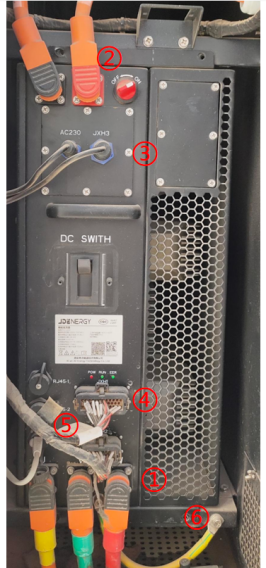
\includegraphics[width=0.2\textwidth]{6.1Sequence for Plugging and Unplugging the PCS Connection Cable.png}
    \caption{Sequence for Plugging and Unplugging the PCS Connection Cable}
\end{figure}

\textbf{PCS handling}
During PCS handling, four people must work together. Use specially designed hooks—two long and two short—to lift the PCS. Place the PCS horizontally on the ground with the radiator side facing down. Use the short hooks to engage the mounting holes on the front side, and use the long hooks on the back side to secure the fins.
\begin{figure}[H]
    \centering
    % 固定图片高度，确保两张图显示等高
    \begin{tabularx}{\textwidth}{@{} >{\centering\arraybackslash}m{0.49\linewidth} @{} @ {\hspace{0.02\textwidth}} >{\centering\arraybackslash}m{0.49\linewidth} @{}}
        
        % 第一张图
        \adjustbox{center}{
            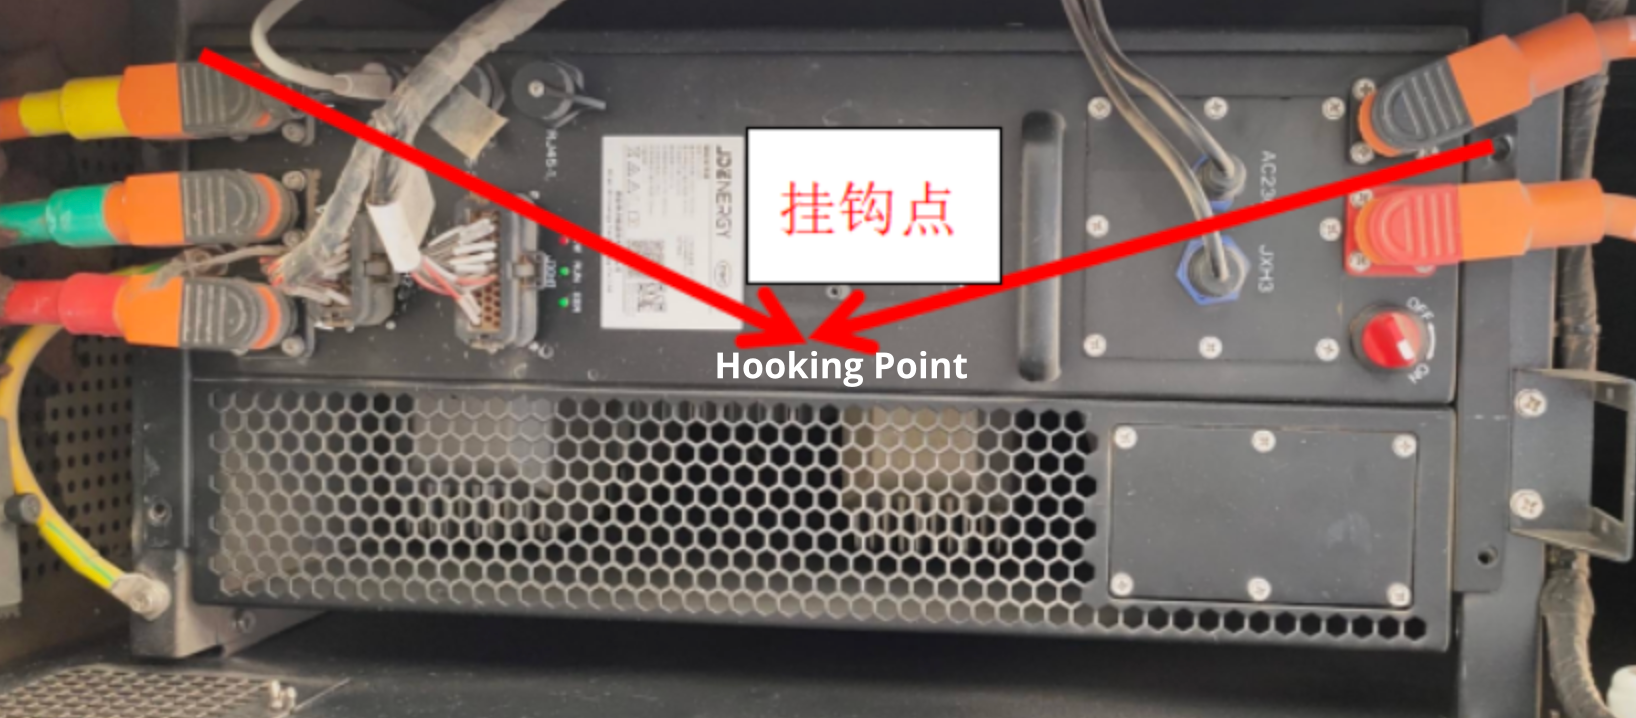
\includegraphics[width=\linewidth,height=4.5cm]{6.2Front Layout of PCS.png}
        }
        \captionof{figure}{Front Layout of PCS} % 注意这里改用 captionof
        & 
        % 第二张图
        \adjustbox{center}{
            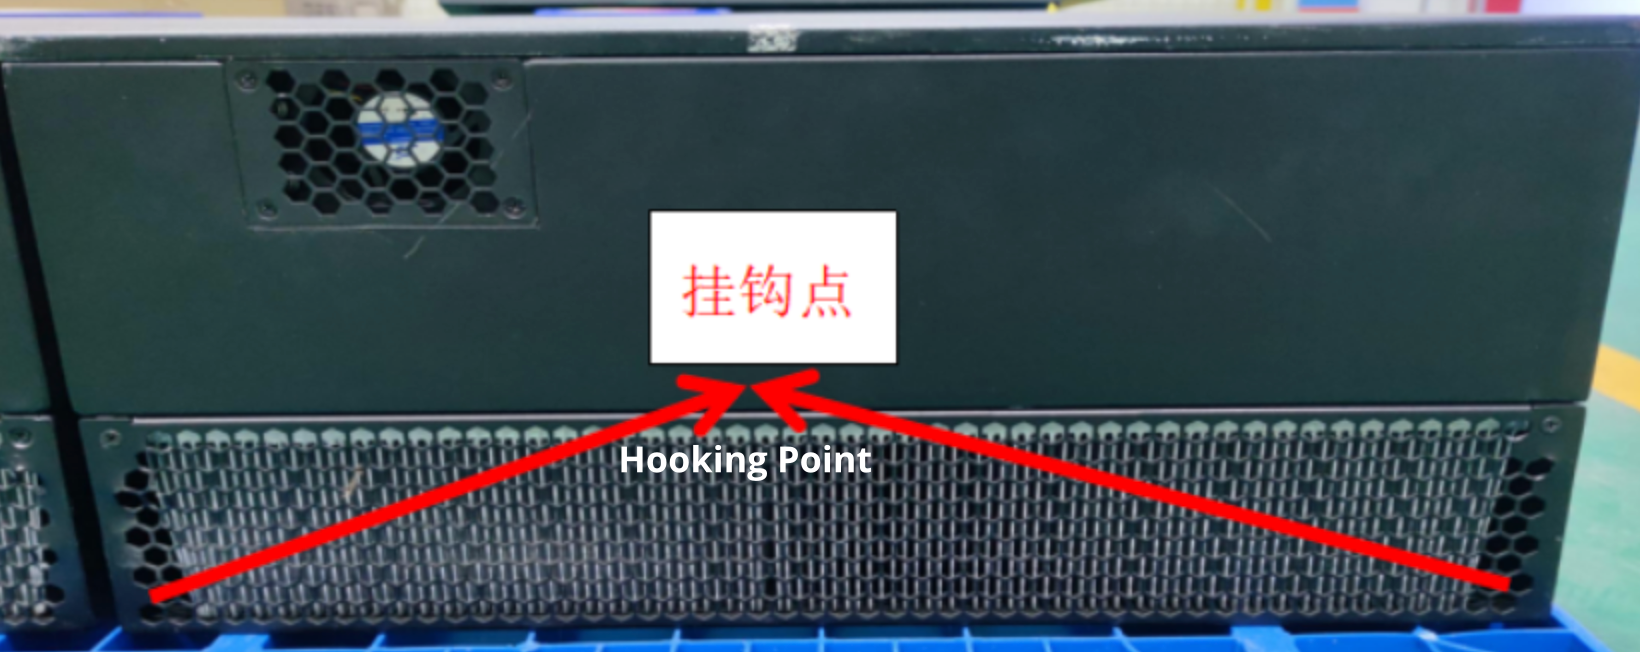
\includegraphics[width=\linewidth,height=4.5cm]{6.3Backside Layout of the PCS.png}
        }
        \captionof{figure}{Backside Layout of the PCS}
        \label{fig:back_layout}
        
    \end{tabularx}
\end{figure}

{\renewcommand\tabularxcolumn[1]{m{#1}}
\begin{tabularx}{\textwidth}{>{\centering\arraybackslash}m{0.16\textwidth} >{\raggedright\arraybackslash}m{0.18\textwidth} >{\raggedright\arraybackslash}X}
\toprule

\includegraphics[height=3.2em]{warning.png} & \symname{Warning} & \symdesc{It is strictly forbidden to use hooks to hang the fan inlet, otherwise the fan will be damaged.}\\
\bottomrule
\end{tabularx}
}



\textbf{PCS installation and commissioning}

After the newly replaced PCS has been installed, connect the cable terminals in the following sequence:

\begin{enumerate}[leftmargin=1.5em]
    \item Install the grounding cable from the PCS to the cabinet.
    \item Install the four fixing screws.
    \item Install the JXH2 connector and the auxiliary AC 230V connector on the PCS.
    \item Install the multi-strand terminal harness connectors JXH1 and JXH2 on the PCS.
    \item Connect the RJ45-3 network cable from the PCS to the switch in the control cabinet.
    \item Connect the DC cable from the battery measurement point to the PCS measurement point.
    \item Install the main power cable for the PCS.
\end{enumerate}

After the cable installation is complete, connect the auxiliary power supply to the PCS, upgrade the PCS program, and configure the parameters.

{\renewcommand\tabularxcolumn[1]{m{#1}}
\begin{tabularx}{\textwidth}{>{\centering\arraybackslash}m{0.16\textwidth} >{\raggedright\arraybackslash}m{0.18\textwidth} >{\raggedright\arraybackslash}X}
\toprule

\includegraphics[height=3.2em]{warning.png} & \symname{Warning} & \symdesc{When removing the screws from the battery cell, it is strictly forbidden to use tools that have not been insulated to prevent short circuits and electric arc burns.} \\
\bottomrule
\end{tabularx}
}

\subsection{PACK Fault Part Replacement}
When a cell failure or sampling line fault occurs and it becomes necessary to remove the PACK battery pack for repair, follow these steps:
\begin{enumerate}[leftmargin=1.5em]
    \item Shut down the PCS equipment.
    \item Drain the coolant from the equipment.
    \item Disconnect the cables connected to the faulty PACK.
    \item Remove the MSD from the PACK.
    \item Disconnect the inlet and outlet pipes of the water-cooling system on the PACK.
    \item Remove the mounting screws of the PACK.
    \item Install appropriate-sized pull rings at the screw holes of the PACK.
    \item Pull out the PACK.
\end{enumerate}

\begin{figure}[H]
    \centering
    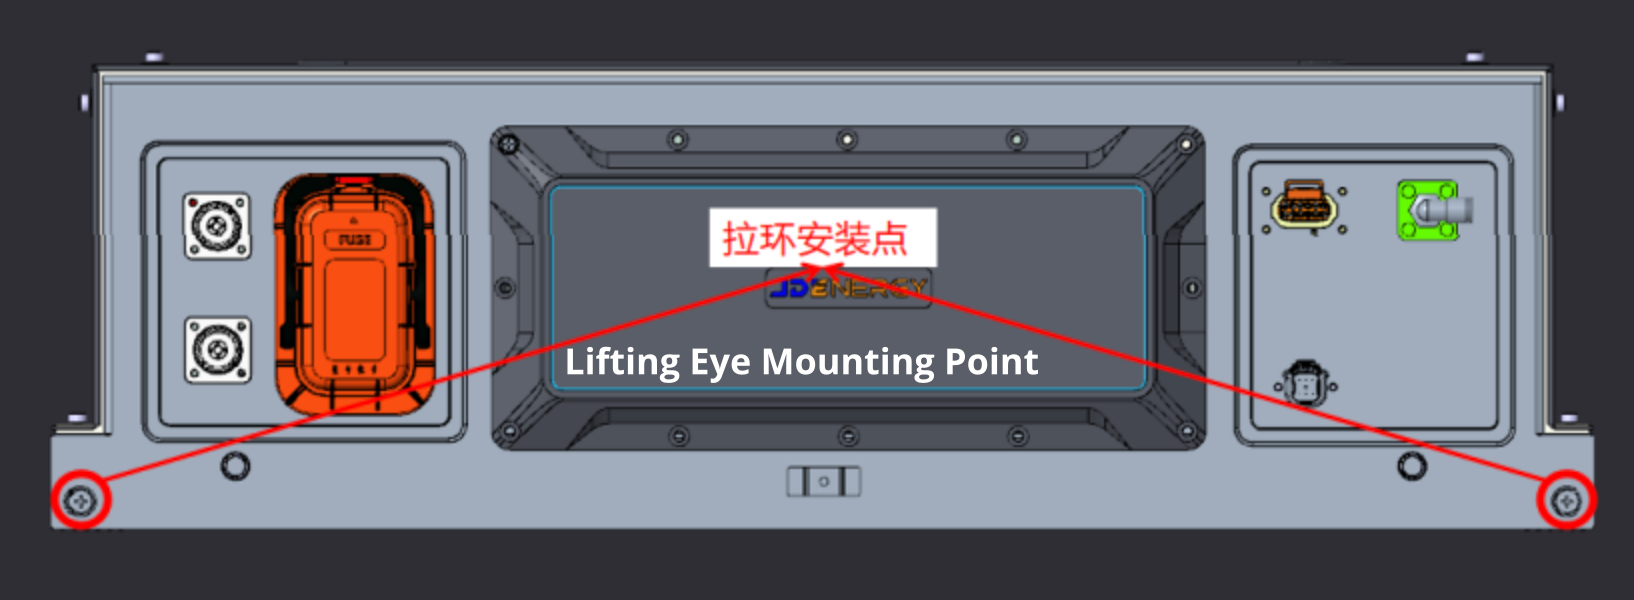
\includegraphics[width=0.8\textwidth, height=5cm, keepaspectratio]{6.4Front view of the PACK battery pack.png}
    \caption{Front view of the PACK battery pack}
\end{figure}

After removing the PACK cover and inspecting the voltage and temperature sampling wires, be careful not to damage the blue film or the insulating film. It is strictly prohibited to use tools to simultaneously touch both the positive and negative terminals of the battery cells.

\begin{itemize}[leftmargin=1.5em]
    \item After opening PACK cover, protect all insulation films and sampling harnesses from mechanical damage.
    \item Never use tools to contact battery positive and negative terminals simultaneously.
    \item Use only insulated tools when removing cell screws to prevent short-circuit and arc burn.
\end{itemize}

\subsection{BMUP\_52S Fault Board Replacement}
When an abnormality is detected in the cell or temperature sampling, and the debugging personnel confirm that the BMUP board is faulty, the replacement procedure is as follows:
\begin{enumerate}[leftmargin=1.5em]
    \item Remove the CAN communication harness connected to the BMUP board on the corresponding PACK.
    \item Use an M5 Allen wrench to remove the front-panel screws.
    \item Remove the BMUP board's outer casing along with its mounting screws.
    \item Replace the BMUP board.
\end{enumerate}

% --- 图 6.5: 居中大图 ---
\begin{figure}[H]
    \centering
    % 增加宽度至 0.8，作为章节引导图
    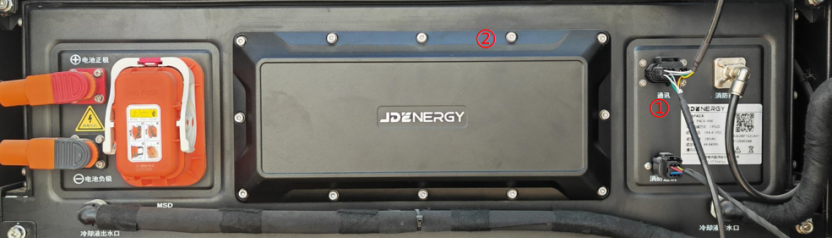
\includegraphics[width=0.8\textwidth, height=5cm, keepaspectratio]{6.5PACK Front Panel Installation and Removal.png}
    \caption{PACK Front Panel Installation and Removal}
    \label{fig:pack_panel}
\end{figure}

\vspace{1em} % 增加一点呼吸间距

\begin{figure}[H]
    \centering
    % 使用 m{宽度} 确保两列的中轴线对齐
    \begin{tabularx}{\textwidth}{@{} >{\centering\arraybackslash}m{0.49\linewidth} @{\hspace{0.02\textwidth}} >{\centering\arraybackslash}m{0.49\linewidth} @{}}
        
        % --- 第一张图 ---
        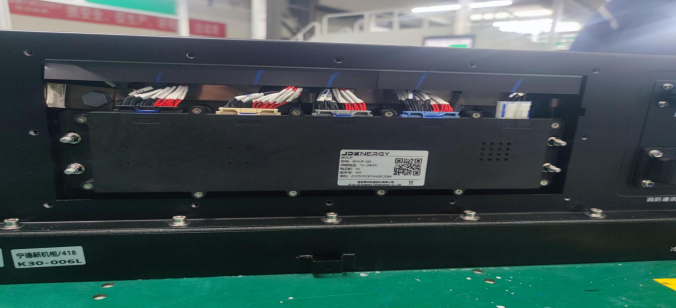
\includegraphics[width=\linewidth,height=4.5cm]{6.6Removal of the BMUP Housing.png}
        \captionof{figure}{Removal of BMUP Housing}
        & 
        % --- 第二张图 ---
        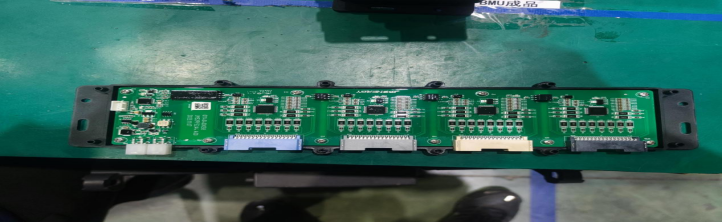
\includegraphics[width=\linewidth,height=4.5cm]{6.7BMUP Board Replacement.png}
        \captionof{figure}{BMUP Board Replacement}
        \label{fig:bmup_replacement}
        
    \end{tabularx}
\end{figure}

After the BMUP board has been replaced, proceed with the BMUP board ID setting and parameter modification.

\clearpage
% ==========================================
% Chapter 9: Technical Support and Warranty Information
% ==========================================
\section{Technical Support and Warranty Information}

\subsection{Technical Support}
If issues occur during operation or maintenance, contact technical support with detailed fault symptoms, station information, and equipment serial numbers.
\begin{itemize}[leftmargin=1.5em]
    \item Customer Service: 400-1336580 / 029-84845916
    \item Email: customer@jdenergy.com
    \item Website: http://www.jd-energy.com.cn
\end{itemize}

\subsection{Warranty Terms}
\textbf{Warranty period}

This energy storage cabinet is covered by a limited warranty for [warranty period] years from the date of purchase.

\textbf{Warranty coverage}

Under normal use, free repair or part replacement is provided for failures caused by product quality issues. The following are excluded from warranty coverage:
\begin{itemize}[leftmargin=1.5em]
    \item Damage caused by improper operation or human factors (collision, water ingress, unauthorized modification, etc.).
    \item Damage caused by natural disasters or force-majeure events.
    \item Problems caused by failure to install, use, or maintain the product according to this manual.
\end{itemize}

\textbf{Warranty process}

If warranty service is required, contact customer service first and provide detailed fault symptoms and equipment information. Preliminary remote troubleshooting will be performed. If on-site or return-to-factory service is required, follow the provided service instructions and prepare supporting documents (e.g., purchase receipt and product manual).

\clearpage

\section*{Appendix I: Inspection and Patrol Form}
\addcontentsline{toc}{section}{Appendix I: Inspection and Patrol Form}
\clearpage
I. Basic Inspection Record Form

% 定义旋转表头命令
\newcommand{\vhead}[1]{\rotatebox{90}{\sffont\small #1}}

\begin{xltabular}{\textwidth}{|c|p{1.8cm}|p{1.3cm}|X|c|c|l|l|l|l|}
\hline
\textbf{No.} & \textbf{Content} & \textbf{Cycle} & \centering\textbf{Abnormal Conditions} & \textbf{Deadline} & \textbf{Method} & \vhead{Result} & \vhead{Action} & \vhead{Date} & \vhead{Staff} \\ \hline
\endfirsthead

\hline
\textbf{No.} & \textbf{Content} & \textbf{Cycle} & \centering\textbf{Abnormal Conditions} & \textbf{Deadline} & \textbf{Method} & \vhead{Result} & \vhead{Action} & \vhead{Date} & \vhead{Staff} \\ \hline
\endhead

% --- 第1组：基础 (使用 Multirow 合并) ---
\hline
\multirow{6}{*}{1} & \multirow{6}{*}{Foundation} & \multirow{6}{*}{\makecell{Once / \\ 6 Mon}} & Settlement, displacement, or tilting exceeding design. & 1 Mon & Reinforce & & & & \\ \cline{4-10}
 & & & Concrete base cracking, peeling, or pulverization. & 1 Mon & Repair & & & & \\ \cline{4-10}
 & & & Base surface damage exposing anchor bolts/steel bars. & 1 Mon & Repair & & & & \\ \cline{4-10}
 & & & Damaged or loose load-bearing parts/bolts; weld cracks. & 1 Mon & Repair & & & & \\ \cline{4-10}
 & & & Loose or damaged module blocks. & 1 Mon & Fix & & & & \\ \cline{4-10}
 & & & Supporting structures affecting system safety/operation. & 1 Mon & Adjust & & & & \\ \hline

% --- 第2组：防腐 ---
2 & Anti-corr. & Once / 6 Mon & Peeling or corrosion of protective coatings on metal. & 1 Week & Repaint & & & & \\ \hline

% --- 第3组：接地 ---
3 & Grounding & Once / Year & Abnormal grounding position; resistance $> 4\Omega$. & 1 Week & Reweld & & & & \\ \hline

% --- 第4组：其他 ---
4 & Other & Once / 6 Mon & Any other anomalies affecting system safety. & -- & -- & & & & \\ \hline

\end{xltabular}


\clearpage

II. AC distribution cabinet inspection record form

\renewcommand{\vhead}[1]{\rotatebox{90}{\sffont\small #1}}

\begin{xltabular}{\textwidth}{|c|p{2.0cm}|p{1.5cm}|X|c|c|c|c|c|c|}
\hline
\textbf{No.} & \textbf{Content} & \textbf{Cycle} & \centering\textbf{Abnormal Conditions} & \textbf{Deadline} & \textbf{Method} & \vhead{Result} & \vhead{Action} & \vhead{Date} & \vhead{Staff} \\ \hline
\endfirsthead

\hline
\textbf{No.} & \textbf{Content} & \textbf{Cycle} & \centering\textbf{Abnormal Conditions} & \textbf{Deadline} & \textbf{Method} & \vhead{Result} & \vhead{Action} & \vhead{Date} & \vhead{Staff} \\ \hline
\endhead

\multicolumn{10}{r}{\textit{Continued on next page...}} \\ \hline
\endfoot
\hline
\endlastfoot

% --- 1. Visual Inspection ---
\hline
\multirow{2}{*}{1} & \multirow{2}{*}{\makecell[l]{Visual \\ Inspection}} & \multirow{2}{*}{Routine} & Deformation, corrosion, leakage, or dust accumulation. & 1 Week & \makecell{Repair/ \\ Clean} & & & & \\ \cline{4-10}
 & & & Damaged safety warning signs/labels. & 1 Week & Replace & & & & \\ \hline

% --- 2. Indicators ---
2 & Indicators & Routine & Abnormal power, position, or fault indicator lights. & 1 Week & \makecell{Repair/ \\ Replace} & & & & \\ \hline

% --- 3. Temperature ---
3 & Temperature & Routine & Abnormal temperature of components. & 1 Week & \makecell{Repair/ \\ Replace} & & & & \\ \hline

% --- 4. Control Loop ---
4 & \makecell[l]{Control \\ Circuits} & During Outage & Loose connections or terminals. & Promptly & Tighten & & & & \\ \hline

% --- 5. Protection Settings ---
5 & \makecell[l]{Protection \\ Settings} & 1 Year & Deviation or change in protection settings. & Promptly & Calibrate & & & & \\ \hline

% --- 6. Circuit Breaker ---
6 & \makecell[l]{Circuit \\ Breaker} & 1 Year & Unable to operate or mechanical failure. & Promptly & \makecell{Repair/ \\ Replace} & & & & \\ \hline

% --- 7. Transformers ---
\multirow{3}{*}{7} & \multirow{3}{*}{Transformer} & \multirow{3}{*}{6 Months} & Abnormal sound or odor from the transformer body. & 1 Mon & Repair & & & & \\ \cline{4-10}
 & & & Dust accumulation on bushing or insulators. & Promptly & Clean & & & & \\ \cline{4-10}
 & & & Cracks or damage to ceramic components. & 1 Mon & Repair & & & & \\ \hline

% --- 8 & 9. Relay & Characteristic Tests ---
8 & \makecell[l]{Relay \\ Protection} & 3 Years & Non-compliant device action characteristics. & 1 Week & \makecell{Factory \\ Tuning} & & & & \\ \hline
9 & \makecell[l]{Switchgear \\ Tests} & 6 Years & Non-compliant withstand voltage or resistance. & 1 Week & \makecell{Report \\ for Tech} & & & & \\ \hline

% --- 10 & 13. Lightning Protection (Merged as requested) ---
\multirow{2}{*}{10} & \multirow{2}{*}{\makecell[l]{Lightning \\ Protection}} & \multirow{2}{*}{\makecell[l]{Before \\ Storms}} & Device failure or invalidation. & 1 Week & Replace & & & & \\ \cline{4-10}
 & & & SPD window discoloration or counter increase. & 1 Week & Replace & & & & \\ \hline

% --- 11. Monitoring Data ---
11 & \makecell[l]{Monitoring \\ System} & Routine & Data deviation $>5\%$ or communication interruption. & Promptly & \makecell{Factory \\ Tuning} & & & & \\ \hline

% --- 12. Power Quality ---
12 & \makecell[l]{Power \\ Quality} & 6 Months & Power quality does not meet relevant standards. & -- & Report & & & & \\ \hline

% --- 14, 15, 16. Enclosure Internal ---
14 & \makecell[l]{Cable \\ Inlets} & 1 Month & Damage or corrosion at cable entry bends. & 1 Week & \makecell{Insulate/ \\ Anti-rust} & & & & \\ \hline
15 & \makecell[l]{Internal \\ Enclosure} & 1 Month & Traces of water ingress or internal corrosion. & 1 Week & \makecell{Drain/ \\ Anti-rust} & & & & \\ \hline
16 & \makecell[l]{Fasteners} & 1 Month & Loose mounting screws or bolts. & Promptly & Tighten & & & & \\ \hline

% --- 17. Internal Fuses ---
17 & \makecell[l]{Fuses \& \\ Breakers} & 6 Months & Excessive voltage drop or loss in fuses/breakers. & 1 Week & Replace & & & & \\ \hline

% --- 18. Other ---
18 & Others & 6 Months & Any other observed anomalies. & -- & -- & & & & \\ \hline

\end{xltabular}

\clearpage
III. Converter Inspection Record Form

\renewcommand{\vhead}[1]{\rotatebox{90}{\sffont\small #1}}

\begin{xltabular}{\textwidth}{|c|p{1.8cm}|p{1.5cm}|X|c|c|c|c|c|c|}
\hline
\textbf{No.} & \textbf{Content} & \textbf{Cycle} & \centering\textbf{Abnormal Conditions} & \textbf{Deadline} & \textbf{Method} & \vhead{Result} & \vhead{Action} & \vhead{Date} & \vhead{Staff} \\ \hline
\endfirsthead

\hline
\textbf{No.} & \textbf{Content} & \textbf{Cycle} & \centering\textbf{Abnormal Conditions} & \textbf{Deadline} & \textbf{Method} & \vhead{Result} & \vhead{Action} & \vhead{Date} & \vhead{Staff} \\ \hline
\endhead

\multicolumn{10}{r}{\textit{Continued on next page...}} \\ \hline
\endfoot
\hline
\endlastfoot

% --- 1. System Operating Status ---
\multirow{3}{*}{1} & \multirow{3}{*}{\makecell[l]{Operating \\ Status}} & \multirow{3}{*}{Routine} & Converter casing damage or deformation. & -- & Report & & & & \\ \cline{4-10}
 & & & Significant vibration or abnormal noise during operation. & -- & Report & & & & \\ \cline{4-10}
 & & & Abnormal overheating of the converter casing. & -- & Report & & & & \\ \hline

% --- 2. Cleaning ---
2 & Cleaning & Routine & Dust accumulation on surface; inlet/outlet blockage. & Promptly & Clean & & & & \\ \hline

% --- 3. Electrical Connection ---
\multirow{2}{*}{3} & \multirow{2}{*}{\makecell[l]{Electrical \\ Connection}} & \multirow{2}{*}{Routine} & Loose cable connections. & Promptly & Tighten & & & & \\ \cline{4-10}
 & & & Cuts or damage on cable insulation in contact with metal. & 3 Days & \makecell{Insulation \\ Wrap} & & & & \\ \hline

% --- 4. Warning Signs ---
4 & \makecell[l]{Warning \\ Signs} & Routine & Damaged, curled, or detached warning labels. & 1 Week & Repair & & & & \\ \hline

% --- 5. Fans ---
\multirow{3}{*}{5} & \multirow{3}{*}{Fans} & \multirow{3}{*}{Routine} & Excessive vibration or abnormal noise during fan operation. & 1 Week & \makecell{Lubricate/ \\ Clean} & & & & \\ \cline{4-10}
 & & & Cracks on fan blades. & 1 Week & Replace & & & & \\ \cline{4-10}
 & & & Blocked or dirty air filter in the enclosure. & 1 Week & Clean & & & & \\ \hline

% --- 6. Circuit Breaker ---
6 & \makecell[l]{Circuit \\ Breaker} & Routine & Abnormal AC/DC breaker or switch failure. & 3 Days & Replace & & & & \\ \hline

% --- 7. Terminals ---
7 & Terminals & Routine & Loose or broken input/output terminals. & Promptly & \makecell{Tighten/ \\ Replace} & & & & \\ \hline

% --- 8 & 9. Power Quality & Faults ---
8 & \makecell[l]{Power \\ Quality} & Routine & Output power quality exceeds standard limits. & -- & Report & & & & \\ \hline
9 & \makecell[l]{Fault \\ Check} & Routine & System function error reported. & Promptly & \makecell{Consult \\ Factory} & & & & \\ \hline

% --- 10. Lightning Protection ---
10 & \makecell[l]{Lightning \\ Prot.} & \makecell[l]{Stormy \\ Season} & Surge protection device (SPD) invalidation. & 3 Days & Replace & & & & \\ \hline

% --- 11. Temperature ---
11 & \makecell[l]{Enclosure \\ Temp.} & Routine & Abnormal temperature of internal components. & 1 Week & \makecell{Repair/ \\ Replace} & & & & \\ \hline

% --- 12. Grounding Test ---
12 & \makecell[l]{Grounding \\ Test} & 1 Year & Grounding resistance between adjacent devices $> 0.2\Omega$. & 1 Week & Repair & & & & \\ \hline

% --- 13. Smart Monitoring ---
13 & \makecell[l]{Monitoring} & Routine & Data deviation $>5\%$ (V, I, f, T) or comms interruption. & 3 Days & \makecell{Calibrate/ \\ Repair} & & & & \\ \hline

% --- 14. Indicators ---
14 & \makecell[l]{Indicator \\ Lights} & Routine & Power, operation, or device fault indicators abnormal. & Promptly & \makecell{Check \\ Logs} & & & & \\ \hline

% --- 15. Interior ---
15 & Interior & Routine & Foreign objects inside the cabinet. & Promptly & Clean & & & & \\ \hline

% --- 16. Busbars ---
16 & \makecell[l]{Busbars \& \\ Interface} & Routine & Loose or blackened busbar/breaker connections. & Promptly & Tighten & & & & \\ \hline

% --- 17. Fuses ---
17 & \makecell[l]{Breakers \& \\ Fuses} & \makecell[l]{Routine \\ (Spot)} & Voltage drop or loss does not meet manufacturer reqs. & 1 Week & Replace & & & & \\ \hline

% --- 18. Other ---
18 & Others & 6 Months & Any other observed anomalies. & -- & -- & & & & \\ \hline

\end{xltabular}
\clearpage


IV. Isolation Transformer Inspection Record Form
\renewcommand{\vhead}[1]{\rotatebox{90}{\sffont\small #1}}

\begin{xltabular}{\textwidth}{|c|p{1.8cm}|p{1.5cm}|X|c|c|c|c|c|c|}
\hline
\textbf{No.} & \textbf{Content} & \textbf{Cycle} & \centering\textbf{Abnormal Conditions} & \textbf{Deadline} & \textbf{Method} & \vhead{Result} & \vhead{Action} & \vhead{Date} & \vhead{Staff} \\ \hline
\endfirsthead

\hline
\textbf{No.} & \textbf{Content} & \textbf{Cycle} & \centering\textbf{Abnormal Conditions} & \textbf{Deadline} & \textbf{Method} & \vhead{Result} & \vhead{Action} & \vhead{Date} & \vhead{Staff} \\ \hline
\endhead

\multicolumn{10}{r}{\textit{Continued on next page...}} \\ \hline
\endfoot
\hline
\endlastfoot

% --- 1. Support Insulator ---
1 & \makecell[l]{Support \\ Insulator} & Routine & Discharge marks or other abnormal phenomena. & -- & Report & & & & \\ \hline

% --- 2. Isolation Transformer Sound ---
2 & \makecell[l]{Iso-Trans. \\ Sound} & Routine & Abnormal "humming" or noise from isolation transformer. & -- & Report & & & & \\ \hline

% --- 3. Leads, Cables, Busbars ---
3 & \makecell[l]{Leads \& \\ Busbars} & Routine & Abnormal heating of lead joints, cables, or busbars. & Promptly & \makecell{Check for \\ Short/Ground} & & & & \\ \hline

% --- 4. Control/Terminal Boxes ---
4 & \makecell[l]{Control \\ Boxes} & \makecell[l]{Monthly / \\ Post-Rain} & Dampness; abnormal operation of temperature control devices. & 1 Week & \makecell{Moisture- \\ proofing} & & & & \\ \hline

% --- 5. Fans ---
5 & \makecell[l]{Fans \& \\ Blowers} & 1 Month & Poor operation or mechanical obstruction. & 3 Days & \makecell{Repair/ \\ Replace} & & & & \\ \hline

% --- 6. Temp. Controller ---
6 & \makecell[l]{Temp. \\ Controller} & 1 Month & Data inconsistency; unbalanced 3-phase temp; high temp alarm. & 3 Days & \makecell{Contact \\ Factory} & & & & \\ \hline

% --- 7. Insulation Resistance ---
7 & \makecell[l]{Insulation \\ Resistance} & \makecell[l]{Before \\ Operation} & Non-compliant with DL/T 596 pre-test regulations. & -- & Rectify & & & & \\ \hline

% --- 8. Box-type Monitor ---
8 & \makecell[l]{Box-type \\ Monitoring} & Routine & Data deviation $>5\%$ (V, I, f, P); communication interruption. & 3 Days & \makecell{Calibrate/ \\ Repair} & & & & \\ \hline

% --- 9. Arrester ---
9 & \makecell[l]{Lightning \\ Arrester} & Routine & Record the counter readings of the lightning arrester. & -- & \makecell{Replace if \\ necessary} & & & & \\ \hline

% --- 10. Others ---
10 & Others & 1 Month & Any other observed anomalies. & -- & -- & & & & \\ \hline

\end{xltabular}
\clearpage

V. Cable Inspection Record Form

\renewcommand{\vhead}[1]{\rotatebox{90}{\sffont\small #1}}

\begin{xltabular}{\textwidth}{|c|p{1.8cm}|p{1.5cm}|X|c|c|c|c|c|c|}
\hline
\textbf{No.} & \textbf{Content} & \textbf{Cycle} & \centering\textbf{Abnormal Conditions} & \textbf{Deadline} & \textbf{Method} & \vhead{Result} & \vhead{Action} & \vhead{Date} & \vhead{Staff} \\ \hline
\endfirsthead

\hline
\textbf{No.} & \textbf{Content} & \textbf{Cycle} & \centering\textbf{Abnormal Conditions} & \textbf{Deadline} & \textbf{Method} & \vhead{Result} & \vhead{Action} & \vhead{Date} & \vhead{Staff} \\ \hline
\endhead

\multicolumn{10}{r}{\textit{Continued on next page...}} \\ \hline
\endfoot
\hline
\endlastfoot

% --- 1. Cable Inlets ---
1 & \makecell[l]{Cable \\ Inlets} & 6 Months & Presence of holes or gaps with diameter $> 10$ mm. & Promptly & Sealing & & & & \\ \hline

% --- 2. Support Points ---
2 & \makecell[l]{Cable \\ Supports} & 6 Months & Damaged or incomplete cable support points. & 3 Days & Tightening & & & & \\ \hline

% --- 3. Electrical Shaft ---
3 & \makecell[l]{Electrical \\ Shaft} & 6 Months & Foreign objects or water accumulation in the shaft. & 1 Week & \makecell{Clean \& \\ Drain} & & & & \\ \hline

% --- 4. Indoor Trench ---
4 & \makecell[l]{Indoor \\ Trench} & 1 Year & Damaged cable outer insulation/sheath. & Promptly & \makecell{Insulation \\ Wrapping} & & & & \\ \hline

% --- 5. Buried Cables ---
5 & \makecell[l]{Buried \\ Cables} & 1 Year & Excavation, heavy loads, or corrosive discharge near the path. & 1 Week & Removal & & & & \\ \hline

% --- 6. Outdoor Trench ---
6 & \makecell[l]{Outdoor \\ Trench} & 1 Year & Damaged covers; water/debris; loose/rusty brackets; rusty armor. & 1 Week & \makecell{Clean \& \\ Anti-rust} & & & & \\ \hline

% --- 7. Connectors ---
7 & \makecell[l]{Cable \\ Connectors} & 6 Months & Poor contact, water ingress, deformation, or overheating. & Promptly & \makecell{Clean \& \\ Tighten} & & & & \\ \hline

% --- 8. Cable Terminals ---
8 & \makecell[l]{Cable \\ Terminals} & 6 Months & Terminals placed directly on metal roofs (loose binding). & Promptly & \makecell{Fix \& \\ Secure} & & & & \\ \hline

% --- 9. Outdoor Trays ---
9 & \makecell[l]{Outdoor \\ Trays/Ducts} & 6 Months & Dirty surface; insecure covers; rusty connectors or bolts. & 1 Week & \makecell{Clean \& \\ Anti-rust} & & & & \\ \hline

% --- 10. Joint Temp ---
10 & \makecell[l]{Joint \\ Temp} & 6 Months & Local temp difference $> 15\%$ or $> 10^\circ$C. & 3 Days & \makecell{Check for \\ Faults} & & & & \\ \hline

% --- 11. Others ---
11 & Others & 6 Months & Any other observed anomalies. & -- & -- & & & & \\ \hline

\end{xltabular}
\clearpage

VI. Fire protection system inspection record form

\renewcommand{\vhead}[1]{\rotatebox{90}{\sffont\small #1}}

\begin{xltabular}{\textwidth}{|c|p{1.8cm}|p{1.5cm}|X|c|c|c|c|c|c|}
\hline
\textbf{No.} & \textbf{Content} & \textbf{Cycle} & \centering\textbf{Abnormal Conditions} & \textbf{Deadline} & \textbf{Method} & \vhead{Result} & \vhead{Action} & \vhead{Date} & \vhead{Staff} \\ \hline
\endfirsthead

\hline
\textbf{No.} & \textbf{Content} & \textbf{Cycle} & \centering\textbf{Abnormal Conditions} & \textbf{Deadline} & \textbf{Method} & \vhead{Result} & \vhead{Action} & \vhead{Date} & \vhead{Staff} \\ \hline
\endhead

\multicolumn{10}{r}{\textit{Continued on next page...}} \\ \hline
\endfoot
\hline
\endlastfoot

% --- 1. Gas Fire Extinguishing System Visual Inspection ---
\hline
\multirow{2}{*}{1} & \multirow{2}{*}{\makecell[l]{Gas Fire Ext. \\ Visual Insp.}} & \multirow{2}{*}{1 Month} & Mechanical damage (deformation, corrosion) to storage containers or nozzles; damaged coating/labels; incomplete seals/safety signs. Agent pressure $<$ 90\% of design. & Promptly & Replace & & & & \\ \cline{4-10}
 & & & Pressure of the pneumatic driving device gas source $<$ 90\% of design pressure. & Promptly & Replace & & & & \\ \hline

% --- 2. Full System Inspection ---
2 & \makecell[l]{Full System \\ Inspection} & Quarterly & Loose containers, pipes, or brackets; deformed/cracked/aged high-pressure hoses; blocked nozzles; agent net weight $<$ 90\% of design capacity. & 3 Days & \makecell{Tighten \\ brackets; \\ Pressure \\ tests; \\ Refill/Rep.} & & & & \\ \hline

% --- 3. Simulated Discharge Test ---
3 & \makecell[l]{Simulated \\ Discharge} & 1 Year & Annual simulated discharge test in the protection zone shows abnormal results. & Promptly & \makecell{Meet Design \\ Reqs.} & & & & \\ \hline

% --- 4. Others ---
4 & Others & 6 Months & Any other observed anomalies. & -- & -- & & & & \\ \hline

\end{xltabular}
\clearpage

VII. Energy Storage Battery System Inspection Record Form

\renewcommand{\vhead}[1]{\rotatebox{90}{\sffont\small #1}}

\begin{xltabular}{\textwidth}{|c|p{1.8cm}|p{1.5cm}|X|c|c|c|c|c|c|}
\hline
\textbf{No.} & \textbf{Content} & \textbf{Cycle} & \centering\textbf{Abnormal Conditions} & \textbf{Deadline} & \textbf{Method} & \vhead{Result} & \vhead{Action} & \vhead{Date} & \vhead{Staff} \\ \hline
\endfirsthead

\hline
\textbf{No.} & \textbf{Content} & \textbf{Cycle} & \centering\textbf{Abnormal Conditions} & \textbf{Deadline} & \textbf{Method} & \vhead{Result} & \vhead{Action} & \vhead{Date} & \vhead{Staff} \\ \hline
\endhead

\multicolumn{10}{r}{\textit{Continued on next page...}} \\ \hline
\endfoot
\hline
\endlastfoot

% --- 1. Battery Equipment ---
1 & \makecell[l]{Battery \\ Equipment} & 1 Month & Abnormal appearance of system equipment. Poor contact or corrosion of leads/terminals in battery and distribution parts; unreliable cable/flexible joint connections; aging, scratches, or damage to wires. & Promptly & Replace & & & & \\ \hline

% --- 2. Battery Monitoring ---
2 & \makecell[l]{Battery \\ Monitoring} & 1 Month & Inaccurate detection of voltage, current, or temperature by the Battery Management System (BMS). & Promptly & \makecell{Replace \\ Sensor / \\ Re-calibrate} & & & & \\ \hline

% --- 4. Others ---
3 & Others & 6 Months & Any other observed anomalies. & -- & -- & & & & \\ \hline

\end{xltabular}

\clearpage

VIII. Data Acquisition and Control System Inspection Record Form

\renewcommand{\vhead}[1]{\rotatebox{90}{\sffont\small #1}}

\begin{xltabular}{\textwidth}{|c|p{1.8cm}|p{1.5cm}|X|c|c|c|c|c|c|}
\hline
\textbf{No.} & \textbf{Content} & \textbf{Cycle} & \centering\textbf{Abnormal Conditions} & \textbf{Deadline} & \textbf{Method} & \vhead{Result} & \vhead{Action} & \vhead{Date} & \vhead{Staff} \\ \hline
\endfirsthead

\hline
\textbf{No.} & \textbf{Content} & \textbf{Cycle} & \centering\textbf{Abnormal Conditions} & \textbf{Deadline} & \textbf{Method} & \vhead{Result} & \vhead{Action} & \vhead{Date} & \vhead{Staff} \\ \hline
\endhead

\multicolumn{10}{r}{\textit{Continued on next page...}} \\ \hline
\endfoot
\hline
\endlastfoot

% --- 1. Data Acquisition ---
1 & \makecell[l]{Data Acq. \\ Equipment} & Routine & Abnormal indicator lights or host failure leading to data upload failure. & Promptly & \makecell{Check data/ \\ power lines; \\ cleaning} & & & & \\ \hline

% --- 2. Monitoring Server ---
2 & \makecell[l]{Monitoring \\ Server} & Routine & Slow speed, abnormal CPU/RAM usage, system crash, or rebooting. & Promptly & \makecell{Backup DB; \\ Optimization; \\ Antivirus; \\ Cleaning} & & & & \\ \hline

% --- 3. Terminal Host ---
3 & \makecell[l]{Terminal \\ Host} & Routine & Slow operating speed or abnormal CPU/Memory utilization. & Promptly & \makecell{Optimization; \\ Antivirus; \\ Cleaning} & & & & \\ \hline

% --- 4. Control Software ---
\multirow{2}{*}{4} & \multirow{2}{*}{\makecell[l]{Control \\ Software}} & \multirow{2}{*}{Routine} & Abnormal radiation data displayed on the monitoring page. & Promptly & \makecell{Data \\ Calibration} & & & & \\ \cline{4-10}
 & & & Data frozen, signal alarm failure/false alarm, lost history, or remote control failure. & Promptly & \makecell{Comm. or \\ Software \\ Recovery} & & & & \\ \hline

% --- 5. Video Surveillance ---
5 & \makecell[l]{Video \\ Surveillance} & Routine & No image display; loose/leaking power boxes; loose power cables. & Promptly & \makecell{On-site \\ Repair} & & & & \\ \hline

% --- 6. Others ---
6 & Others & 6 Months & Any other observed anomalies. & -- & -- & & & & \\ \hline

\end{xltabular}
\clearpage

\section*{Appendix II: Emergency Response Measures for Energy Storage Unit Fire}
\addcontentsline{toc}{section}{Appendix II: Emergency Response Measures for Energy Storage Unit Fire}

\subsection*{Event Characteristics}
\addcontentsline{toc}{subsection}{Event Characteristics}

\begin{enumerate}[label=\arabic*., leftmargin=2em]
    \item \textbf{Risk Analysis and Event Types:} 
    Internal insulation damage leading to short circuits, or violation of operating procedures (e.g., using open flames in the enclosure) may cause battery ignition. Battery fires pose a severe threat to personnel and equipment safety, potentially leading to casualties or the complete destruction of the energy storage unit.

    \item \textbf{Target Area and Equipment:} Energy Storage Unit Clusters (e-Block Area).

    \item \textbf{High-Risk Periods and Hazard Levels:}
    \begin{itemize}
        \item \textbf{Seasons/Timing:} High-temperature summer (high-load operation), windy spring and autumn seasons, or periods of deteriorating equipment insulation.
        \item \textbf{Hazards:} 
        \begin{itemize}
            \item Battery cabinet explosions leading to personnel casualties.
            \item Interruption of power supply to associated electrical equipment and lines.
            \item Damage to site equipment, loss of power generation, and property damage.
            \item Casualties caused by personnel misoperation.
        \end{itemize}
    \end{itemize}

    \item \textbf{Pre-incident Signs:}
    \begin{itemize}
        \item High-load operation in summer heat causing insulation aging, leading to breakdown, ignition, and explosion.
        \item Frequent fault alarms reported by a specific unit on the HMI/Background monitoring system.
    \end{itemize}
\end{enumerate}

\subsection*{Field Emergency Response Procedures}
\addcontentsline{toc}{subsection}{Field Emergency Response Procedures}
Upon fire outbreak, the primary mission is fire suppression, personnel rescue, and protection of critical assets.

\begin{enumerate}[label=\arabic*., leftmargin=2em]
    \item \textbf{Notification:} The witness must immediately notify the Team Leader with details of the fire scale.
    \item \textbf{External Aid:} The Team Leader coordinates a call to local fire departments (119) and reports the situation to the Emergency Office and Regional Management.
    \item \textbf{Evacuation:} The Team Leader and Safety Officer must evacuate personnel to a safe zone and establish a \textbf{100-meter exclusion zone} centered on the unit.
    \item \textbf{Isolation:} The Team Leader contacts the control room operator to de-energize the circuit connected to the affected unit.
    \item \textbf{Suppression:} Await fire department arrival for professional firefighting.
    \item \textbf{Status Report:} After extinguishment, the Team Leader reports the final status to the management.
    \item \textbf{Evidence Preservation:} Protect the scene for subsequent accident investigation.
    \item \textbf{Review:} Conduct a preliminary analysis meeting to summarize the handling process and update records.
\end{enumerate}

\subsection*{Field Emergency Response Measures}
\addcontentsline{toc}{subsection}{Field Emergency Response Measures}
\begin{itemize}[label=\checkmark]
    \item Operators or site electricians must immediately isolate and \textbf{shut down the power supply} to the energy storage area.
    \item The emergency team must quickly assess the scene, organize on-site rescue, and determine if external 119 aid is required.
    \item Evacuate all personnel near the unit. \textbf{Do not approach the affected e-Block.}
    \item If there are casualties, conduct rescue only if the safety of the rescuers is fully guaranteed.
    \item If controllable, organize firefighting using designated facilities (e.g., external water spray) and contact the system manufacturer.
\end{itemize}

\subsection*{Safety Notes}
\addcontentsline{toc}{subsection}{Safety Notes}
\begin{tcolorbox}[colback=red!5!white,colframe=red!75!black,title=Critical Warnings]
\begin{itemize}[leftmargin=1.2em, nosep]
    \item \textbf{Post-Event Recovery:} Protect the scene and evidence. Work may only resume after relevant authorities approve the safety measures.
    \item \textbf{Plan Optimization:} Scientifically summarize the entire process to correct deficiencies in the Emergency Plan.
    \item \textbf{Preventative Analysis:} Identify patterns from the accident to implement targeted safety measures.
    \item \textbf{Resource Replenishment:} Immediately replenish consumed first-aid supplies, tools, and spare parts after the site is cleared.
    \item \textbf{Night Operation:} Provide adequate lighting if rescue occurs at night or in low-visibility environments.
    \item \textbf{Personal Safety:} Rescuers must prioritize their own safety at all times.
\end{itemize}
\end{tcolorbox}

\end{document}
